\documentclass[USenglish]{ifimaster}  %% ... or USenglish or norsk or nynorsk
\usepackage[utf8]{inputenc}           %% ... or latin1
\usepackage[T1]{fontenc,url}
\usepackage{todonotes}
\urlstyle{sf}
\usepackage{babel,textcomp,duomasterforside,varioref,graphicx}
\usepackage[backend=biber,style=numeric-comp]{biblatex}
\usepackage{acronym}
\usepackage{amsmath , amssymb , amsthm}
%\usepackage[margin=1.2in, footskip=0.25in]{geometry}
\usepackage{float}
\usepackage{listings}
\usepackage{minted}
\usepackage{xcolor}
\usemintedstyle{autumn}
\usepackage{mathtools}
\usepackage[export]{adjustbox}
\usepackage{svg}
\usepackage{pdfpages}
\usepackage[toc,page]{appendix}
\usepackage{tabularx}
\usepackage{todonotes}
\usepackage{listings}
\usepackage[wby]{callouts}
\usepackage{subcaption}
\usepackage[hidelinks]{hyperref}
\usepackage{cleveref}
\usepackage[toc,page]{appendix}
\usepackage{csquotes}
\usepackage[section]{placeins}

%\graphicspath{ {Images/} } 
%\setlength{\parskip}{1em}
%\setlength{\parindent}{0em}
%\linespread{1.5}
%\newcommand{\myparagraph}[1]{\paragraph{#1}\mbox{}\\}
%\usetikzlibrary{arrows.meta,
%               chains,
%                positioning,
%                shapes.geometric
%                }

\definecolor{LightGray}{gray}{0.95}

\lstset{
  language=bash,
  basicstyle=\ttfamily
}

% Den kommandoen under bestemmer hvor mye som skal være inkuldert i table of contents
%\setcounter{tocdepth}{5}

\title{Image-based terrain characterization for autonomous vehicles, based on deep learning}        %% ... or whatever

\author{Andreas Hagen}                      %% ... or whoever 

\bibliography{references.bib}                  %% ... or whatever



\begin{document}

\duoforside[dept={Department of Physics},   %% ... or your department
  program={Electronics and Computer Technology Program option: Cybernetics},  %% ... or your programme
  short]                                        %% ... or long

\frontmatter{}
\chapter*{Abstract}                   %% ... or Sammendrag or Samandrag
For an autonomous vehicle to interpret and understand the scene in front of itself, it relies on several types of different sensors. A camera may be one of these sensors, and through implementing a \acf{cnn} it is possible to extract all the necessary features from the images. To be able to extract the desired features, the network needs ground truth for some images to train itself with a supervised learning method.

This thesis seeks to investigate the opportunity to partly automate the process of generating ground truth for all images in a terrain-based scene. To generate ground truth for a single image may take from two minutes to over an hour depending on the scene and the number of classes. The ground truth does in this context consist of two classes in the form of road and background. Two datasets without ground truth containing 439 and 2040 images are used in this project, 45 and 164 images respectively are manually labeled and act as ground truth for the training set in each dataset. The network's mission is further to predict the ground truth for the remaining 2270 images automatically after it has executed the training.

The residual network implemented in this thesis manages to some extent to provide most of the images with somewhat close to an accepted ground truth. The exceptions are the most demanding scenes where objects arrive in the scene. This problem may be solved by adding more classes to the objects with the highest probability for arriving in the scene. The residual network does, therefore, lack some robustness to predict well in all types of scenes. 

\chapter*{Sammendrag}
For at et autonomt kjøretøy skal kunne tolke og forstå miljøet foran seg selv, trenger den hjelp av flere typer forskjellige sensorer. Et kamera kan være en slik sensor, og gjennom implementering av et konvolusjonelt nevralt nettverk er det mulig å trekke ut alle nødvendige egenskaper fra bildene. For å trekke ut de ønskede egenskapene, trenger nettverket fasiten fra noen av bildene, så det kan trene seg opp gjennom ledet-læring.

Denne avhandlingen ønsker å undersøke muligheten til å delvis automatisere prosessen med å generere fasiten for alle bildene i et terrengbasert miljø. Å generere fasiten til ett enkelt bilde kan ta alt fra to minutter til over en time avhengig av antall klasser og hvordan scenen ser ut. Fasiten i denne oppgaven består av to klasser i form av vei og bakgrunn. Det er brukt to datasett uten fasit i denne oppgaven, hvor det første inneholder 439 bilder og det andre 2040 bilder. Videre er det generert fasit manuelt til 45 bilder fra det første datasettet og til 164 bilder fra det andre datasettet, hvor disse bildene er plassert i treningssettet. Nettverkets oppgave er dermed å forutsi fasiten til de resterende 2270 bildene automatisk etter det har utført treningen.   

Det nettverket med best resultat i denne oppgaven, greier til en viss grad å forutse en tolkning som kan aksepteres som en slags fasit til de fleste bildene. Unntakende er de mest krevende miljøene hvor det ankommer forskjellig objekter i scenen. Dette problemet kan løses ved å legge til flere klasser i form av de objektene som har størst sannsynlighet for å dukke opp i scenen. Det beste nettverket i avhandlingen mangler med andre ord noe robusthet for å kunne forutse fasiten til bildene i samtlige typer miljø. 

\chapter*{Preface}


\tableofcontents{}
\listoffigures{}
\listoftables{}

\chapter*{Abbreviations}
%\addcontentsline{toc}{chapter}{Abbreviations} \noindent
%--- Acronyms -----------------------------------------------------------------%
% \acrodef{label}[acronym]{written out form} % acronym syntax
%\acrodef{etacar}[$\eta$ Car]{Eta Carinae}   % acronym example
%--- Acronyms -----------------------------------------------------------------%
% how to use acronyms:
% \ac = use acronym, first time write both, full name and acronym
% \acf = use full name (text + acronym)
% \acs = only use acronym
% \acl = only use long text
% \acp, acfp, acsp, aclp = use plural form for acronym (append 's')
% \acsu, aclu = write + mark as used
% \acfi = write full name in italics and acronym in normal style
% \acused = mark acronym as used
% \acfip = full, emphasized, plural, used
%--- Acronyms -----------------------------------------------------------------%
\begin{acronym}
        \acro{ugv}[UGV]{unmanned ground vehicle}
        \acro{ai}[AI]{artificial intelligence}
        \acro{ann}[ANN]{artificial neural network}
        \acro{cnn}[CNN]{convolutional neural network}
        \acro{fcn}[FCN]{fully convolutional network}
        \acro{dl}[DL]{deep learning}
        \acro{ml}[ML]{machine learning}
        \acro{cpu}[CPU]{central processing unit}
        \acro{gpu}[GPU]{graphics processing unit}
        \acro{gui}[GUI]{graphical user interface}
        \acro{rgb}[RGB]{red, green, blue}
        \acro{iou}[IoU]{intersection over union}
        \acro{miou}[mIoU]{mean intersection over union}
\end{acronym}


\mainmatter{}
\chapter{Introduction}
\todo{Legg til hva tidligere forskning har oppnådd(I introduksjonen skal du plassere deg i fagfeltet og vise at du har kjennskap til tidligere forskning. Introduksjonen skal gjøre rede for hva vi vet og hva vi ikke vet om feltet.)}
This section will provide an introduction to the thesis starting with the motivation, before covering the problem formulation and describing the goals of the thesis. Lastly, the thesis outline is explained. 
\section{Motivation}
An \ac{ugv} needs several different sensor inputs to understand the entire scene in front of itself, and further provide its software with the necessary information to make the right decisions where to drive or not. One of these sensors can be in the form of a \ac{rgb}-camera mounted on the vehicle.

This thesis will take two raw terrain datasets from a \ac{rgb}-camera, and investigate if it is possible to predict the ground truth in the images by classifying each pixel in the image as either road or background. A raw dataset will in this context refer to a dataset containing only images without any ground truth providing the correct answers to the classifications.

\section{Problem formulation}
Convolutional neural networks (described in \cref{cnn}) are nowadays able to perform object detection with an accuracy similar to the human level \cite{website:cnn}. Performing that well, the \ac{cnn} is a robust choice of a network for image-based data. Most of the \acp{cnn} has the same thing in common; They train with supervised learning on large datasets, containing many ground truth images. However, in some cases, the dataset at hand may consist of only raw images without any ground truth. To manually label a dataset, can be a time-consuming task, and to automate this task would save both time and costs. The problem formulation in this thesis consists therefore of the following sentence:
\begin{itemize}
\centering
  \item[] \textbf{Will the use of \acp{cnn} provide useful test set predictions in a raw terrain-image dataset, given only a few manually annotated images?} 
\end{itemize}

Two different \acp{cnn} will be implemented in order to automate the task of labeling the datasets. This thesis will investigate if the predictions made by the networks can be used as ground truth for the images in the datasets. Unlike in most other datasets, this problem formulation seeks to only use a few manually labeled images in the training set. Even though most \acp{cnn} use large datasets with many annotated images in the training set, François Chollet argues in his book \textit{"Deep Learning with Python"} that \ac{dl} can be applicable to fairly small datasets as well \cite{Francois_Deep_learning_with_python}. 

\section{Contribution and goals}
The implementation of the first network (the residual) in the thesis is loosely based on the contribution from Ronneberger, Fischer, and Brox in their invention of the U-Net \cite{website:u_net_article}. 
\begin{figure}[ht]
    \centering
    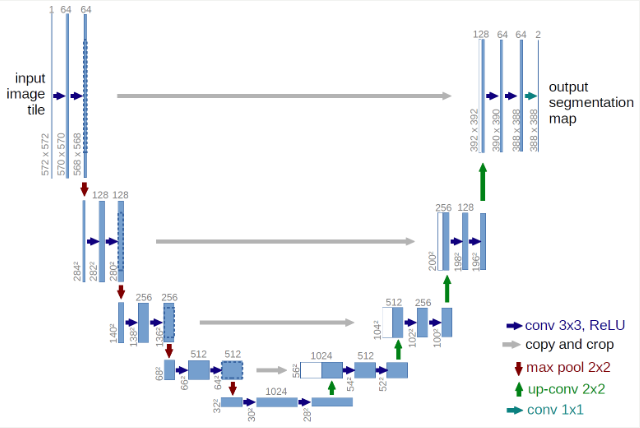
\includegraphics[width=0.8\textwidth]{bilder/u_net.png}
    \caption{The structure of the U-Net \cite{website:u_net}}
    \label{fig:u_net}
\end{figure}
The U-Net was initially a \ac{cnn} meant for biomedical image segmentation. The main features in the network consists of its \textit{"Skipping connections"} marked with grey arrows as \textit{"copy and crop"} in \cref{fig:u_net}. Imagine the \textit{"U-shape"} being split at the shortest grey arrow in the bottom, the part to the left would then be the contraction part, while the part to the right would be the expansion part. The \textit{"Skipping connections"} concatenates the features from the contraction part with the corresponding up-convolutions in the expansion part. The U-Net architecture made it possible to gain very good results based on few training samples, and that is exactly the type of feature which is desired in this thesis.

This part of the section describes the goals in the thesis, which are as follows:
\begin{itemize}
    \item \textbf{Perform a literature review of existing \acp{cnn} and choose a robust network to implement}
    \item \textbf{Implement a very basic \ac{cnn} in addition, to use as baseline}
    \item \textbf{Investigate if the \acp{cnn} predictions are good enough to be used as ground truth for the images in the datasets}
    \item \textbf{Gain a more generalized network with transfer learning from a similar dataset}
    \item \textbf{Make two different versions of the training set}
    \item \textbf{Test the networks, present the results, and analyze them}
\end{itemize}

\section{Thesis outline}
\begin{itemize}
    \item \textbf{Chapter 1:}
    \newline
    Presents the thesis introduction including the problem formulation, the contribution and the goals
    \item \textbf{Chapter 2:}
    \newline
    Covers the necessary background theory and the related work
    \item \textbf{Chapter 3:}
    \newline
    Describes the method used and the experiments done
    \item \textbf{Chapter 4:}
    \newline
    Presents the training results, the quantitative results, and the qualitative results
    \item \textbf{Chapter 5:}
    \newline
    Covers the discussion, concludes the thesis and present suggestions for further work
\end{itemize}


\chapter{Theoretical background}
This chapter will initially provide a short overview of the basics of \ac{ai}, \ac{ml}, computer vision, and \acf{dl}. A \ac{dl} framework is used for implementing the network in the thesis, while a few computer vision techniques is used for processing the images further after the predictions. The reasoning behind choosing \ac{dl} will be briefly discussed. Further is the necessary data preprocessing described, before the basics of different \ac{ann} is covered. Lastly, this section will go through the theory of generating ground truth labels with a suitable program.

\section{Artificial intelligence}
\ac{ai} is a field where machines are able to demonstrate intelligence through mathematics, statistics and logic. \ac{ai} has the ability to tackle many complex problems, which are intellectually difficult or impossible to solve for a human being (with natural intelligence). Even though \ac{ai} could solve complex problems, it still had a few challenges in the early days. Some intuitive tasks for humans, such as recognizing a cat or a dog in an image, or the context of a written text, proved to be a true challenge. A solution to these problems was to allow machines to learn from experience, which is where \ac{ml} and \ac{dl} comes into the picture \cite{The_holy_grail_of_DL}.

\begin{figure}[ht]
    \centering
    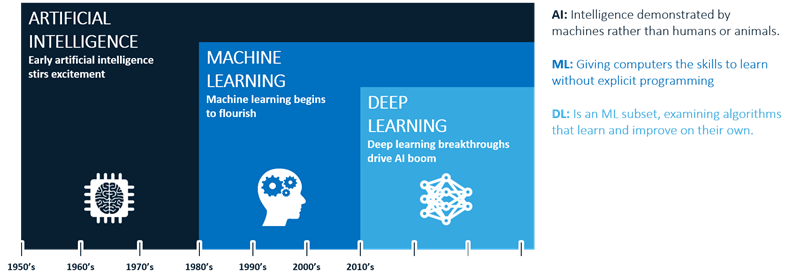
\includegraphics[width=0.8\textwidth]{bilder/AI_ML_DL.png}
    \caption{A provisional timeline for AI, ML, and DL \cite{website:AI}}
    \label{fig:AI}
\end{figure}

\subsection{Machine learning}
\Cref{fig:AI} illustrates that \ac{ml} is a subset from \ac{ai}. The term is further well defined by \ac{ml} pioneer Tom M. Mitchell:
\newline
\newline
\textit{“Machine learning is the study of computer algorithms that allow computer programs to automatically improve through experience.”} \cite{tom_mitchell}.
\newline
\newline
\ac{ml} algorithms will explicitly be programmed to improve their performance on a task. Humans would provide the data, along with the answers in order to search for and produce the rules. This is visualized in \cref{fig:ml} \cite{Francois_Deep_learning_with_python}.
\begin{figure}[ht]
    \centering
    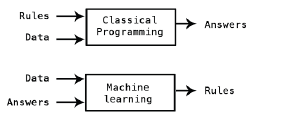
\includegraphics[width=0.8\textwidth]{bilder/ml.png}
    \caption{Classical \ac{ai} illustrated on the top and \ac{ml} illustrated on the bottom part of the image \cite{Francois_Deep_learning_with_python}}
    \label{fig:ml}
\end{figure}

Even though \ac{ml} techniques is not used explicitly in this thesis, it is combined with \ac{ai} the foundation for \ac{dl}.

\subsection{Deep learning}
As visualized in \cref{fig:AI}, \ac{dl} is a subset of both \ac{ai} and \ac{ml}. The main difference between \ac{ml} and \ac{dl} is that \ac{dl} is able to learn data representations from datasets instead. The whole network is in other words able to solve the problem from start to end without using external methods as in \ac{ml}. \ac{dl} has its networks (called \ac{ann}) loosely based on the same principle as the neuron system from a human brain. This thesis will use \ac{dl} as foundation for solving the task of automatically predict ground truth images. 

\subsubsection{Supervised learning}
Supervised learning is the most commonly used technique in \ac{dl} \cite{Francois_Deep_learning_with_python}. The word supervised refers to known targets or annotations in the form of a labelled dataset. With that knowledge a function can learn how to map input data to the targets.

\subsection{Benefits using \ac{dl} with \ac{cnn} vs traditional methods}
\ac{dl} has become increasingly more popular during the last few years. One of the reasons for this increased popularity is \acp{dl} ability to provide higher accuracy when trained with large amounts of data. Even though \ac{dl} is usually known for predicting good results from large datasets, it does also contain methods for providing good results from networks trained with smaller datasets as well. As is the case in this thesis. This benefit over traditional \ac{ml} methods alone would be enough to consider taking \ac{dl} as preferred method.

Another argument for employing \ac{dl} over traditional methods is the features extraction from images. While the traditional algorithms needs to manually implement different computer vision techniques in order to extract the desired features before classification, this is not the case with \ac{dl}. With the use of convolution layers from \ac{cnn} the features are extracted automatically from the layers.
The first layer will detect and learn small edges. Then the second layer will learn larger patterns made from the features from the first layer, and this concept will repeat itself in the further layers. The patterns learned are translation-invariant, which means it can recognize the learned pattern if it appears anywhere else in the image. This advantage are exclusively for the \acp{cnn}, and makes the networks able to generalize better with less training samples than for example a densely-connected network \cite{Francois_Deep_learning_with_python}.

\section{Computer vision}
Computer vision is a field whose main purpose is to make machines able to interpret and understand features from images or video. In other words, "Teaching computers how to see" \cite{website:maskinsyn-intro}. This section will only go through a small number of computer vision concepts, as they are used in the thesis.

\subsection{Semantic segmentation}
Segmentation is a concept where the input is in the form of an image, and the output consists of regions and structures based on the input. Normal segmentation will in most cases only provide a basic scene understanding. If we want to understand what is in the image more thoroughly, semantic segmentation is the next step. The idea behind semantic segmentation is that instead of regions, every pixel in the image are classified. This means that it will be possible to gain a broader scene understanding of the environment in the image, making it easier to recognize different elements \cite{website:semantic_segmentation}.

\subsection{Morphological operations}
A common binary image operations is called \textit{morphological operations}, since
they change the shape of the underlying binary objects \cite{Ritter}. These operations are typically used to clean up binary images. Two of the standard binary morphological operations used in the thesis are: 
\newline
\begin{itemize}
    \item \textbf{Erosion}
    \item \textbf{Dilation}
\end{itemize}

\textit{erosion} thins the object and \textit{dilation} thickens the object. Using these operations in this specific order (erosion + dilation) results in \textit{opening}. This operation tends to smooth boundaries, while also removing some noise from the image. It is common to experiment on how much iteration that should be implemented in each the erosion and the dilation operation.

The structuring element used is normally a square rectangular kernel of desired size. It can also take the shape of an circle if necessary. This depends on what the regions in the image looks like. Sometimes a circle shaped kernel may be a better option to smooth the curves than the normal rectangular kernel.

\subsection{Connected component analysis}
The connected component analysis is a tool, which can be used to filter out noise from a binary image. It labels all the connected regions in the image automatically in an iterative manner. That way it is possible to mask out every label which contains less pixels than a given threshold. If the region after the noise filtering contain holes surrounded by a complete polygon, these can be sealed with a binary object filler. If both operations are implemented successfully, the improvement from the original prediction will be significantly better.

\section{Data preprocessing}
This section will cover data processing from an image-based point of view. Before the dataset can be fed into the network, it would in most cases be inevitable to perform several preprocesses. This is necessary in order to make the data prepared for training. 
\newline
A common thing to do with an image-based dataset is to resize the images to a slightly lower resolution. This is especially necessary if the computer does not have a state-of-art \ac{gpu}, as the model otherwise might be very slow. The down scaling will help the model to be more effective and less time consuming, at the prize of loosing some features from the original resolution. It is therefore important to test different scales, to find the perfect fit between keeping enough key features and have an effective model.
\newline
A \ac{rgb} image contains integer values in the range from 0-255 in each of its three channels. Because the values of the weights in a neural network are relatively small, it is common practice to normalize the image-array to values between 0-1. Dividing the array with 255 will make that happen. Doing so will prevent slowing down the learning process, as the values from the weights and the array now are in closer range. Casting the array from int to float before normalizing would increase the accuracy even further. This is due to the float division resulting in a more accurate number than int division.

Another process is to check whether the dataset has the correct shape or not. This is necessary because the network needs to know which input shape to expect. The input layer in \textit{Keras} is a tensor which is passed to the first hidden layer. If that input layer does not correspond with the shape of each element in the dataset, the network will not be able to execute. In the case where "Conv2D" layers are used in a \textit{Keras} framework, an input array needs to have the following structure:
\newline
\newline
(height, width, channels)
\newline
\newline
Where height and width refers to the x- and y-coordinates in the image, and channels refers to if the image is binary (channels=1) or \ac{rgb} (channels=3).

\subsection{Data augmentation}
Data augmentation is a helpful tool in order to maintain a more generalized model. It is a method for applying transformations to the training data. When the images are pre-processed with the methods described in this section, the network learns how to cope with slightly different images than the original training set. This is the reason the model have a higher chance of predicting the test images (images that the model never have seen before) with more accuracy. In addition to potentially higher accuracy, the model also has lower risk of overfitting. This sub-section will only cover the most used augmentation techniques.  
\subsubsection{Random cropping}
A popular method in data augmentation is random cropping. Random cropping is sampling a random chosen square box from the original image, and then resize to the original size.
\begin{figure}[ht]
    \centering
    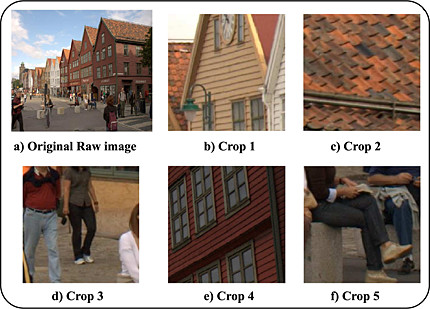
\includegraphics[width=0.8\textwidth]{bilder/random_cropping.png}
    \caption{Random cropping \cite{website:random_cropping}}
    \label{fig:random_cropping}
\end{figure}
As seen in \cref{fig:random_cropping} the image focus on different areas from the original image, due to the random chosen box. This operation must be included with the ground truth images. When an operation changes the geometry in the image, the same operation must be done in the ground truth image in order to still be a valid target. 
\subsubsection{Flipping images}
Another method is to flip the images in either vertical or horizontal order. Even when the images are flipped, are they recognizable for the model. The ground truth must also go through the same operation in order to keep the correct geometry in both images. 
\subsubsection{Color changes}
The idea behind color changes is to make the the model more robust and generalized for new unseen data. Since the geometry in the images are the same after applying color changes, is it not necessary to do any operation on the ground truth images.
\section{Artificial neural networks}
To provide the necessary understanding of how the networks implemented in this thesis works, this section starts by explaining the fundamental pieces of \ac{ann} before diving deeper into \ac{cnn} in \cref{cnn}. Most of the theory in this section is based on the Stanford University course \textit{"CS231n: Convolutional Neural Networks for Visual Recognition"} \cite{website:cs231n}, and from the course \textit{"INF4490 – Biologically Inspired Computing"} \cite{website:inf_4490_slp}\cite{website:inf_4490_mlp} at University of Oslo.

An \ac{ann} is a computing system which is vaguely based on the same principle as biological neurons in a human brain. It has the ability to learn different tasks and data representations. To fully understand the concept, the basics of a neural network is divided into different parts and further described in this section.

\subsection{Single- and multi-layer neural network}
In 1943 McCulloch \& Pitts designed a much simplified version of biological neurons \cite{mcculloch_pitts}. With their design, they are widely known as the inventors of the first \ac{ann}. Their ideas of a threshold in the activation function and combining many basic units in order to increase computational power are still being used today.
\begin{figure}[ht]
    \centering
    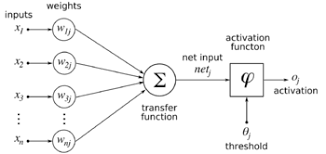
\includegraphics[width=0.8\textwidth]{bilder/mcculloch_and_pitts.png}
    \caption{Illustrates the McCulloch \& Pitts design of a simplified neuron \cite{website:mcCulloch_img}}
    \label{fig:mcculoch_and_pitts}
\end{figure}
The illustration of the neuron and its activation function in \cref{fig:mcculoch_and_pitts} can be mathematically explained with \cref{eq:mcCulloch}.
\begin{equation}\label{eq:mcCulloch}
\begin{aligned}
    {h = \sum_{i=1}^{n} x_i w_i \quad , \quad\quad o =
\begin{cases}
    1 & \text{ h $\geq$ $\theta$ }  \\
    0 & \text{ h < $\theta$ }
\end{cases}}
\end{aligned}
\end{equation}
Where the neurons function ($h$) is denoted in the form of a dot product between the inputs ($x_i$) and the weights ($w_i$). The neurons activation function \textit{"fires"} when the dot product of the input and its weight respectively are higher than a given threshold $\theta$. Meaning the output ($o$) becomes 1 when $h$ is equal to or higher than the threshold, and 0 when $h$ is lower than the threshold value.

If many McCulloch \& Pitts neurons are put together, the structure of a single-layer neural network appears. A single-layer perceptron are able to learn linear problems. When the task is to learn non-linear problems, the solution is to add one or more hidden layers, as done in multi-layer perceptron.   
\begin{figure}[ht]
    \centering
    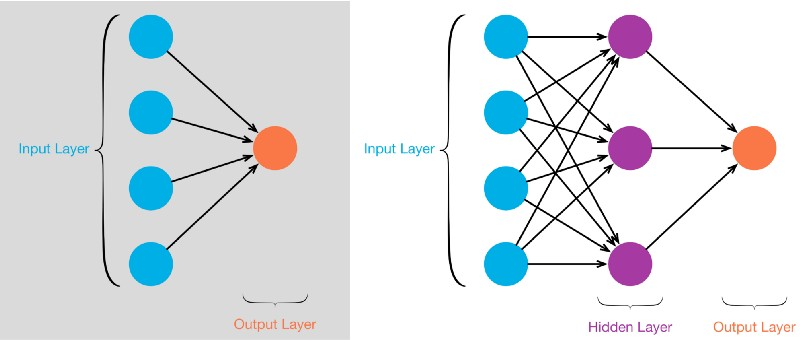
\includegraphics[width=0.8\textwidth]{bilder/slp_&_mlp.jpeg}
    \caption{Single-layer perceptron to the left, and multi-layer perceptron to the right \cite{website:slp_mlp}}
    \label{fig:slp_mlp}
\end{figure}
The difference can be seen visually by \cref{fig:slp_mlp}, where the single-layer perceptron only has an input and an output layer, while the multi-layer perceptron includes at least one hidden layer.

\subsection{The learning rule}
In order for the single-layer neural network to learn, it has to adjust the weights accordingly. This is where the perceptron learning rule become relevant.
\begin{equation}\label{eq:learning_rule}
\begin{aligned}
w_{ij} \longleftarrow w_{ij} + \Delta w_{ij}
\end{aligned}
\end{equation}
\Cref{eq:learning_rule} shows how the weight ($w_{ij}$) updates. The goal of the learning rule is to minimize the error at the output, such that $\Delta w_{ij} = 0 $. When the weights reach that state, they are tuned correctly. The weights can be both positive and negative, and how they adjust can be explained with the next equation. 
\begin{equation}\label{eq:delta_learning_rule}
\begin{aligned}
\Delta w_{ij} = \eta * (t_j - y_j) * x_i 
\end{aligned}
\end{equation}
In \cref{eq:delta_learning_rule} $\eta$ is referred to as the learning rate. It is a scalar which decide how much the weight value in each iteration will change. Finding the right balance in the choice of learning rate is therefore crucial. A high value (e.g. 1) can create an unstable net. With a high learning rate will the weights change a lot every time they updates. %The reason is that the weight will change a lot every time it updates with a high learning rate. 
Choosing a low value will make a stable network, but will require much more learning time, because the weights uses more time to tune into correct values.

$\eta$ is further being multiplied with the error ($(t_j - y_j)$, where $t_j$ is the target output and $y_j$ is the actual output). Before finally being multiplied with the inputs ($x_i$). As stated above, the goal is to minimize this error. Which is done during training where the weights are adjusted with \cref{eq:delta_learning_rule}.
\subsection{Bias}
In the case where all inputs are zero, the weights will have no effect since they are multiplied with the inputs. The solution for that particular case is to have an adjustable threshold, which can be applied with a bias node. The bias node should be added to each neuron. Then \cref{eq:mcCulloch} will become \cref{eq:bias}, where $b$ is the bias.
\begin{equation}\label{eq:bias}
\begin{aligned}
    {h = \sum_{i=1}^{n} x_i w_i + b \quad , \quad\quad o = 
\begin{cases}
    1 & \text{ h $\geq$ $\theta$ }  \\
    0 & \text{ h < $\theta$ }
\end{cases}}
\end{aligned}
\end{equation}
\subsection{Backpropagation in multi-layer neural networks}
When learning in a single-layer neural network, it is possible to gain knowledge about which weight is correct and which is not, as described with the learning rule. In multi-layer perceptron there is at least one hidden layer between the input and the output. Hence, it is impossible to know which weights are correct, and which activations being correct for the neurons in the hidden layer. Without knowing which weight or activation is correct, it is impossible to learn the weights or train the network. The problem of not being able to train a multi-layer neural network was solved in 1986 with an algorithm called backpropagation \cite{Rumelhart:1986:LIR:104279.104293}.
\begin{figure}[ht]
    \centering
    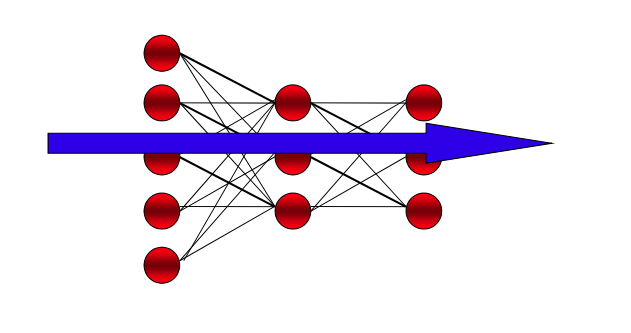
\includegraphics[width=0.8\textwidth]{bilder/forward_prop.png}
    \caption{The forward pass in backpropagation \cite{website:inf_4490_mlp}}
    \label{fig:forward_step}
\end{figure}
The backpropagation algorithm consists of two main steps. The first is the forward pass, which has the following structure illustrated in \cref{fig:forward_step}. After the input layer has received its inputs, the activations of the hidden nodes in the middle layer is calculated. Lastly the activations of the output nodes in the last layer are calculated. 
\begin{figure}[ht]
    \centering
    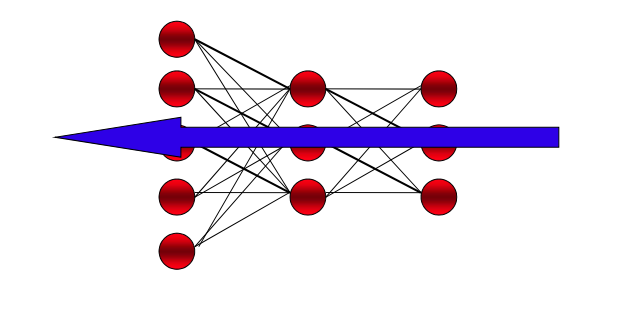
\includegraphics[width=0.8\textwidth]{bilder/backward_prop.png}
    \caption{The backward pass in backpropagation \cite{website:inf_4490_mlp}}
    \label{fig:backward_step}
\end{figure}
The second step in the backpropagation is called the backward pass, and is illustrated in \cref{fig:backward_step}. This step starts by calculating the output errors in the last layer, before it updates the same layers weights. Then the error is being propagated backwards, and the hidden weights in the middle layer are updated. This process is repeated until the first layer is reached.
\subsection{Gradient descent learning and momentum}
When training the network with backpropagation, the goal is to minimize the errors in the network. As described with the backward pass, after being calculated, the errors from the output layer are propagated backwards in the network. The tool used is a form of gradient descent. 
\begin{equation}\label{eq:sum_of_error}
\begin{aligned}
E(w) = \frac{1}{2} \sum_{k}(t_k - y_k)^2 = \frac{1}{2}\sum_{k}(t_k - \sum_{i} w_{ik}x_i)^2
\end{aligned}
\end{equation}
It differentiates the sum-of squares error in \cref{eq:sum_of_error}, showed with the \cref{eq:gradient_descent}.
\begin{equation}\label{eq:gradient_descent}
\begin{aligned}
\Delta w_{ik} = -\eta\frac{\delta E}{\delta w_{ik}}
\end{aligned}
\end{equation}
Even though gradient descent algorithm is a good method for finding the minimum value, it has a potential risk of getting stuck in a local minimum as visualized in \cref{fig:gradient_descent}.
\begin{figure}[ht]
    \centering
    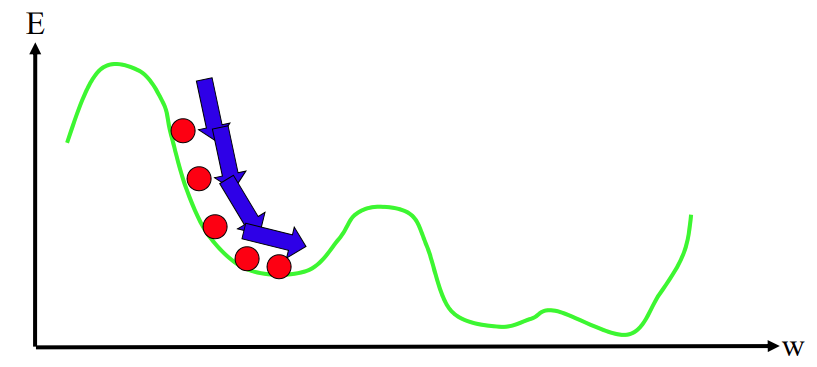
\includegraphics[width=0.8\textwidth]{bilder/gradient_descent.png}
    \caption{Gradient descent \cite{website:inf_4490_mlp}}
    \label{fig:gradient_descent}
\end{figure}
There are two alternatives to avoid being stuck in a local minimum. The first one is to initialize the training several times with random weights. The other method is to use momentum. If the gradient descent algorithm reaches a local minimum, the momentum keeps the algorithm going further uphill for a while, until the descending starts again and hopefully a global minimum will be found instead. Momentum is described mathematically in \cref{eq:momentum}. 
\begin{equation}\label{eq:momentum}
\begin{aligned}
w_{ij} \longleftarrow w_{ij} - \eta\Delta_j z_i+\alpha\Delta w^{t-1}_{ij}
\end{aligned}
\end{equation}
\subsection{Activation functions}
The task of an activation function is to decide whether a neuron should \textit{"fire"} or not. In other words, the activation function takes a number and performs a mathematically operation on it. There exist several activations functions, all with different pros and cons. The ones being used in this thesis will be covered here.
\subsubsection{The sigmoid function}
The sigmoid function was a historically often used activation function. It is mathematically described with \cref{eq:sigmoid}.
\begin{equation}\label{eq:sigmoid}
\begin{aligned}
\sigma(x) = \frac{1}{(1 + e^{-x})}
\end{aligned}
\end{equation}
The function transforms the input numbers into a range between 0-1 as shown in \cref{fig:sigmoid}. This means large negative numbers become 0, while large positive numbers become 1.
\begin{figure}[ht]
    \centering
    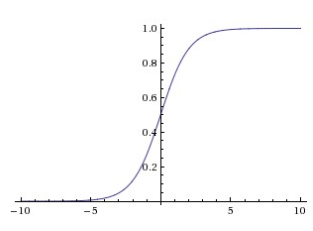
\includegraphics[width=0.6\textwidth]{bilder/sigmoid_function.png}
    \caption{Sigmoid activation function \cite{website:cs231n_activation_functions}}
    \label{fig:sigmoid}
\end{figure}
Today, the popularity of the the sigmoid function has decreased due to the following drawbacks:
\begin{itemize}
    \item \textit{Vanishing gradients at values close to 0 or 1}
    \item \textit{The neurons can be saturated if the initial weights are too large}
    \item \textit{The outputs are not zero-centered}
\end{itemize}

\subsubsection{The ReLu function}
The ReLu function (Rectified Linear Unit) has become increasingly more popular in the last few years. It is proven much faster than the sigmoid or tanh (which is a scaled sigmoid function) functions in a paper, due to its linear, non-saturating form \cite{website:relu}. 

\begin{equation}\label{eq:reLu}
\begin{aligned}
f(x) = max(0,x)
\end{aligned}
\end{equation}

\begin{equation}\label{eq:reLu_2}
\begin{aligned}
{f(x) = 
\begin{cases}
    0 & \text{for x < 0}  \\
    x & \text{for x $\geq$ 0}
\end{cases}}
\end{aligned}
\end{equation}
The ReLu function is described mathematically in two ways in this thesis, both being illustrated in \cref{eq:reLu} and \cref{eq:reLu_2} for a better understanding of the function.

\begin{figure}[ht]
    \centering
    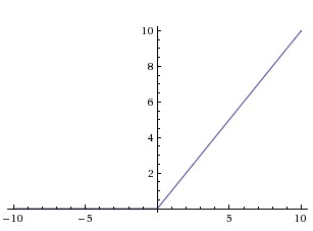
\includegraphics[width=0.6\textwidth]{bilder/relu_activation.png}
    \caption{Relu activation function \cite{website:cs231n_activation_functions}}
    \label{fig:relu}
\end{figure}
As illustrated in \cref{fig:relu} the ReLu activation is thresholded at zero. This makes ReLu a favored choice over the sigmoid/tanh functions. It is a less computationally expensive method, because it does not have the exponential implementation. There is, however, one disadvantage using ReLu. The units can be fragile during training and as much as 40\% of the network may end up \textit{"dead"}. This can happen if a large gradient is flowing through the ReLu neuron. It may cause the neuron to update in such a way that the neuron never will activate on a data point again and end up \textit{"dead"}. With a proper learning rate (not too high), the problem tends to be avoided in most cases.

\subsection{Loss and optimizers}
The task of a loss function is to measure the distance between the predictions being made by the network and the actual ground truth. In this manner there can be computed a distance score, controlling how well the network did with its prediction \cite{Francois_Deep_learning_with_python}. This is illustrated in figure \cref{fig:loss_function}.

\begin{figure}[ht]
    \centering
    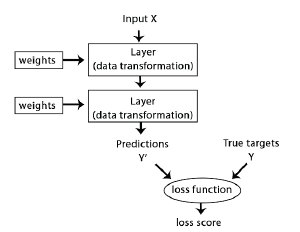
\includegraphics[width=0.6\textwidth]{bilder/loss_function.png}
    \caption{Loss function \cite{Francois_Deep_learning_with_python}}
    \label{fig:loss_function}
\end{figure}
The loss score computed by the loss function, is further being used as a feedback signal for adjusting the weights slightly. The weights are updated in a direction which lower the loss score, in order to make better future predictions. This is shown in \cref{fig:optimizers}. The job of adjusting the weights is executed by what is called an optimizer. The optimizer implements the backpropagation algorithm earlier described in this section \cite{Francois_Deep_learning_with_python}. 

\begin{figure}[ht]
    \centering
    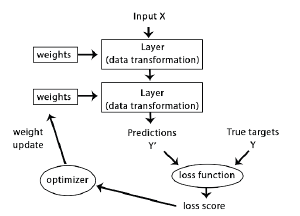
\includegraphics[width=0.6\textwidth]{bilder/optimizers.png}
    \caption{The visualization of an optimizer \cite{Francois_Deep_learning_with_python}}
    \label{fig:optimizers}
\end{figure}


\subsection{Regularization}
To avoid overfitting (explained in page 95 \& 96 \cite{Francois_Deep_learning_with_python}), the implementation of regularization will be helpful. Regularization refers to regulating the weights, by constraining them to only accept small values. It is implemented by adding a \textit{cost} to the loss function if it has too large weights. The cost comes in two different forms:

\begin{itemize}
    \item \textit{\textbf{L1 regularization}}
    \item \textit{\textbf{L2 regularization}}
\end{itemize}
Where \textit{L1 regularization} adds the costs proportionally to the absolute value of the weights coefficients, and \textit{L2 regularization} adds the costs proportionally to the square of the absolute value of the weights coefficients \cite{Francois_Deep_learning_with_python}. 

Another popular regularization method is \textit{dropout}, developed by Hinton and his students at the University of Toronto \cite{website:dropout}. It consists of randomly zeroing out (dropping out) a number of output features of the layer during training. The term \textit{"dropout rate"} refers to the fraction of the features which is being dropped out, and is usually put to a number between 0.2-0.5. When the algorithm is ready for testing, the output values are scaled down with a factor equal to the dropout rate instead of being dropped out. This is done in order to balance for the amount of more active units during testing. To use dropout as a regularization method is both very common and efficient \cite{Francois_Deep_learning_with_python}.   

\subsection{Convolutional neural networks}\label{cnn}
A \ac{cnn} is a sub class of \ac{ann}. It is a type of network which automatically extracts several types of features from images, and are further used for making different sorts of predictions based on the given task. The main difference between a \ac{cnn} and an ordinary neural network is how the input is interpreted. In a \ac{cnn} the inputs is assumed to be images. 

Unlike a \ac{cnn}, an ordinary neural network with fully connected layers will keep all parameters connected from the input until the output. The \ac{cnn}, with the use of convolutions, is able to reduce the numbers of parameters vastly from each layer while keeping the key features. This difference makes \ac{cnn} a better tool for processing images, as images often contains a huge amount of parameters. 

The following example will demonstrate why it is necessary to reduce the parameters when processing images. Imagine an ordinary neural network with an image (width, height, depth) as an input. If the size of the input is (224x224x3) this means the number of weights will become $224 * 224 * 3 = 150528$ weights. Adding more similar neurons will escalate the number of parameters considerably, which then will result in an unnecessary overfitting and a poor network.

The characteristics of a \ac{cnn} is described below, providing a general understanding how the parameters are reduced and \acp{cnn} unique features.

\subsubsection{Convolutional Layer}
Being the core building block of a \ac{cnn}, the convolutional layer does most of the computationally expensive work necessary for the network to perform well. It consists of learnable filters, which slides through the whole input image bit by bit. \Cref{eq:conv} illustrates the general expression of a 1D convolution. Where $\omega$ is the filter being convolved with the input $f(x,y)$, providing the output $g(x,y)$. 

\begin{equation}\label{eq:conv}
\begin{aligned}
g(x,y) = \omega * f(x,y) = \sum_{s=-a}^{a}\sum_{t=-b}^{b}\omega(s,t)f(x-s,y-t)
\end{aligned}
\end{equation}

\begin{figure}[ht]
    \centering
    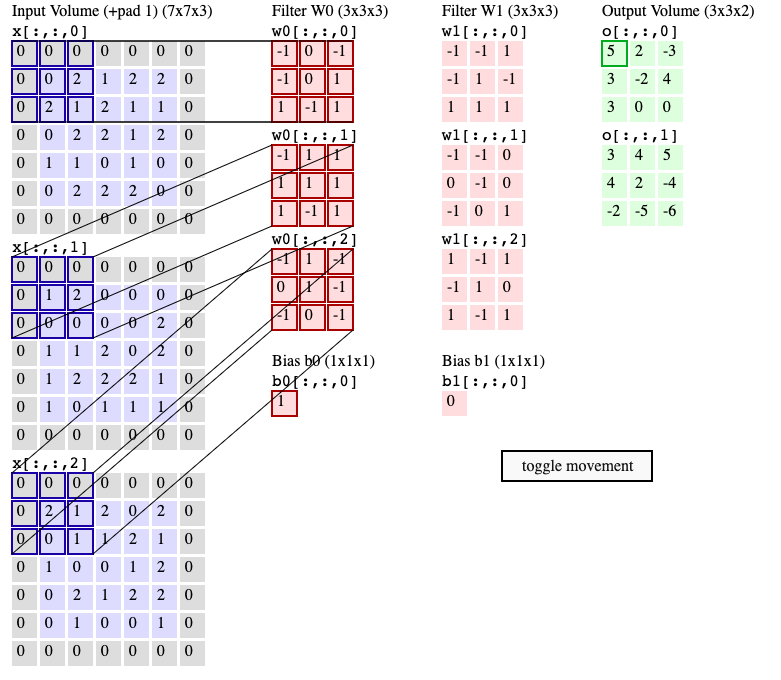
\includegraphics[width=0.8\textwidth]{bilder/conv2.png}
    \caption{3D Convolution step by step \cite{website:cs231n}}
    \label{fig:conv}
\end{figure}
To understand the process even better, the Stanford course \textit{"CS231n: Convolutional Neural Networks for Visual Recognition"} has provided an intuitive visual model showing a 3D convolution explicitly in \cref{fig:conv}. This illustration consists of following parameters and configurations:

\begin{itemize}
    \item \textit{Input volume = (7x7x3)}
    \item \textit{Stride = 2}
    \item \textit{Number of zero padding = 1}
    \item \textit{Two weight filters = (3x3x3)}
    \item \textit{Two biases = (1x1x1)}
    \item \textit{Output volume = (3x3x2)}
\end{itemize}
Where the first weight filter $W_0$ is sliding over each part of the input in its three channels. This gives the output volume O[:,:,0], while the convolving of weight filter $W_1$ provides O[:,:,1]. The stride is set equal to two, which means the filter can slide in three positions both in $x$- and $y$-direction. This operation makes the output dimension into width and height equals to 3. The last dimension in the output volume is set by the amount of filters ($W_0$ and $W_1$) convolving over the input volume. The amount of chosen filters is a hyperparameter and decides the depth of the output. In this example there are two filters, which means the final output volume becomes (3x3x2). 
The implementation of zero padding helps us to control the spatial size of the output. It is also a hyperparameter, and in this example it is set equal to one, which gives us the pad (marked in grey in \cref{fig:conv}) around the input volume filled with zeros. 

The equation to compute the spatial size of the output volume is illustrated in \cref{eq:output_conv}

\begin{equation}\label{eq:output_conv}
\begin{aligned}
O = \frac{(W - F + 2P)}{S}+1
\end{aligned}
\end{equation}
Where $O$ is the output volume. $W$ is the input volume, $F$ is the receptive field (the weight filter), $P$ being the amount of zero padding, and $S$ for the number of strides.
 
\subsubsection{Parameter sharing and local connectivity}
In contrary to ordinary neural networks, \acp{cnn} have neurons set up in three dimensions:
\begin{itemize}
    \item \textit{Width}
    \item \textit{Height}
    \item \textit{Depth}
\end{itemize}
These neurons may have various levels of connectivity between the layers. The two concepts controlling and reducing the amount of connections between the neurons are called parameter sharing and local connectivity. As earlier described, one of the main reason for the \acp{cnn} to out perform ordinary neural networks (when processing images), are their properties to reduce the amount of parameters while keeping key features. 

Parameter sharing means to share some weights and biases in order to control the number of parameters. This can be done by assuming that if a feature is useful to calculate at a specific spatial location ($x_1$,$y_1$), it should be useful to compute it at a different location ($x_2$,$y_2$) as well. In practice that means constraining the neurons in each depth dimension to use the same weights and bias. Parameter sharing will greatly reduce the amount of total weights, and is an important contribute to make an efficient \ac{cnn}. 

Local connectivity connects each neuron only to a small region of the previous layers input, unlike connecting the neurons to all the neurons from the previous layer as done in ordinary neural networks.
This small region is a hyperparameter, and is called the receptive field of the neuron. It is the same as the weight filter from the example above. The depth slice in the weight filter is always the same as the depth slice from the previous layers input. This means that we have local connections along width and height, and full connection along the depth of the input layer.

\subsection{Pooling layer}
Another method to reduce parameters is to add a max pool layer. Similarly to the convolution layer it contains a filter ($F$) and stride ($S$). 

\begin{figure}[ht]
    \centering
    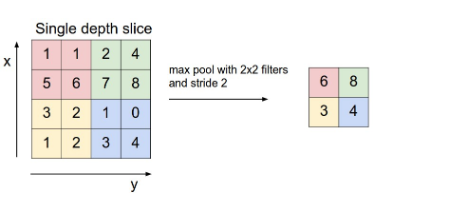
\includegraphics[width=0.8\textwidth]{bilder/max_pooling.png}
    \caption{Max pooling \cite{website:cs231n}}
    \label{fig:max_pooling}
\end{figure}

But as seen in \cref{fig:max_pooling}, the filter takes the max value in each frame instead of convolving through the input like the convolution layer does. The most common values in the max pooling layer are $F=$2 or 3, and $S=2$. Increasing these values will result in a destructive layer. It is a common practice to implement a max pool layer periodically between convolutional layers.

\section{Generating the ground truth labels manually}
There exist several good programs for generating labels for datasets, all with different benefits and shortcomings. The program used in this thesis is a free program, which offer offline annotation. It is called \textit{"labelme"}, and it can be installed directly from GitHub \cite{website:labelme}. The program is easy to learn and contains annotation examples in the GitHub folder. \textit{Labelme} has a clean programmed \ac{gui} regarding the working space, which is illustrated in \cref{fig:annotate}. 

\begin{figure}[ht]
\centering
\begin{subfigure}{.6\textwidth}
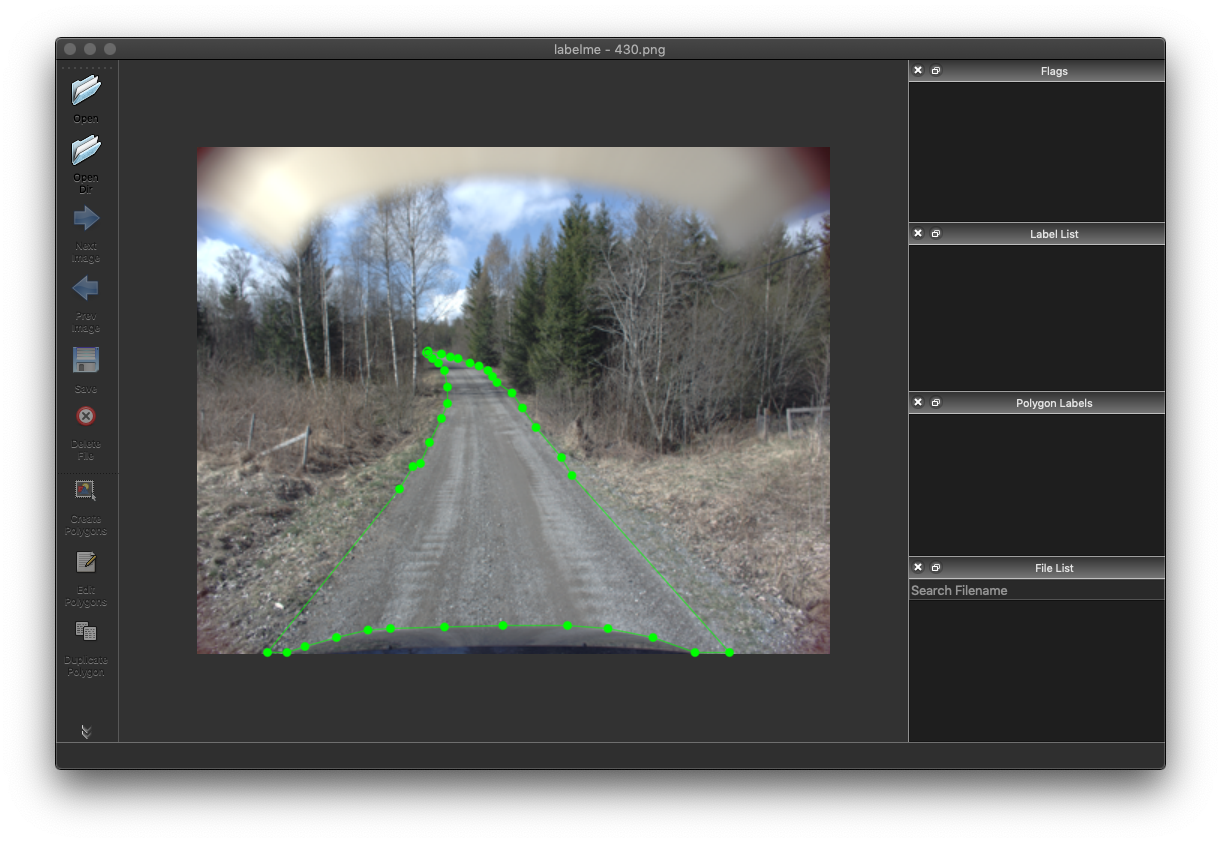
\includegraphics[width=0.7\textwidth]{bilder/annotating.png}
\captionof{figure}{Manually annotating an image with labelme}
\label{fig:annotate}
\end{subfigure}
\begin{subfigure}{.6\textwidth}
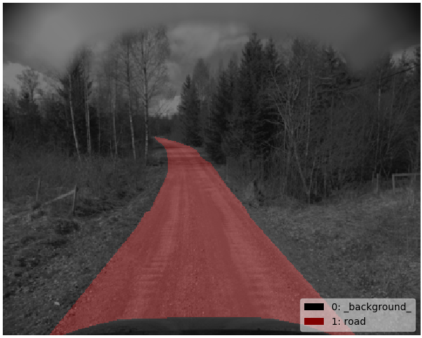
\includegraphics[width=.7\linewidth]{bilder/label_viz.png}
\captionof{figure}{The annotation superimposed on the original image}
\label{fig:finished_annotation}
\end{subfigure}
\caption{Road annotation}
\end{figure}

When the polygon is drawn, another script is run, and the complete annotation ends up like in \cref{fig:finished_annotation}.  

\section{Transfer learning}
Transfer learning applies already learned knowledge from saved weights and applies it to a new problem with a new dataset. It is sometimes referred to as using a pre-trained network. Using a pre-trained network is usually a highly efficient way to gain better results when using small datasets. The spatial features learned by the pre-trained network might prove useful for the original problem the network was designed for, because it may transfer essential knowledge from for example a well made dataset. The results of implementing transfer learning will in most cases provide a much higher accuracy to the original problem, in contrary to only train on a small dataset \cite{Francois_Deep_learning_with_python}. The implementation of transfer learning is therefore used in this thesis due to the very small number of annotated images available for the training set. 

\section{Related work}

\chapter{Method}\label{method}
\section{Implementation}
This chapter will cover the implementation of the program in the thesis and discuss the choices of methods. It will initially describe how the ground truth from the training images is made. Then cover which framework is used, before describing both implementations of \ac{cnn}, with pros and cons. Furthermore the advantage of using Tensorboard will be discussed. The mid section in this chapter will cover predictions made from the network, and a few computer vision techniques used in order to maintain a clean output with minimal noise. The last part of this section will cover the experiments done in this thesis, in the form of describing the structure of the datasets and the training configuration.
\subsection{Annotating the training set}
Before the work with the network can start, there must exist a prepared dataset. As supervised learning is the used method, some of the images needs ground truth in order for the algorithm to maintain a reliable loss function. Only ten percent of the images are manually annotated. This is due to the intention of this thesis to automatically predict the test images ground truth with as little manually annotated images in the training set as possible. The images picked out for manual annotation starts from image number one in the dataset, and continues in an iterative manner every tenth image. The following commands is used in the annotating program \textit{labelme} in order to start and convert the annotation from \textit{.json} to \textit{.png} file format:   

\begin{minted}[bgcolor=LightGray, linenos, fontsize=\footnotesize]{bash}
$ labelme <input_file.png> -O <output_file.json>
$ labelme_json_to_dataset <input_file.json> -o <output_folder>
\end{minted}

When the first line is executed, the \ac{gui} for \textit{labelme} shows up in an external window. From there it is possible to start drawing the annotation by pressing the \textit{"Create Polygons"}. \Cref{fig:polygon} illustrates a finished drawn polygon. After the polygons are drawn and the save button is pressed, the second line is ready to be executed. This command will take all the polygon positions saved in the \textit{.json} file and convert the ground truth into the final \textit{.png} format. The second command will also make a directory which consist of the original image, the ground truth superimposed on the original image, and the ground truth image. 

\begin{figure}[ht]
\begin{subfigure}{.6\textwidth}
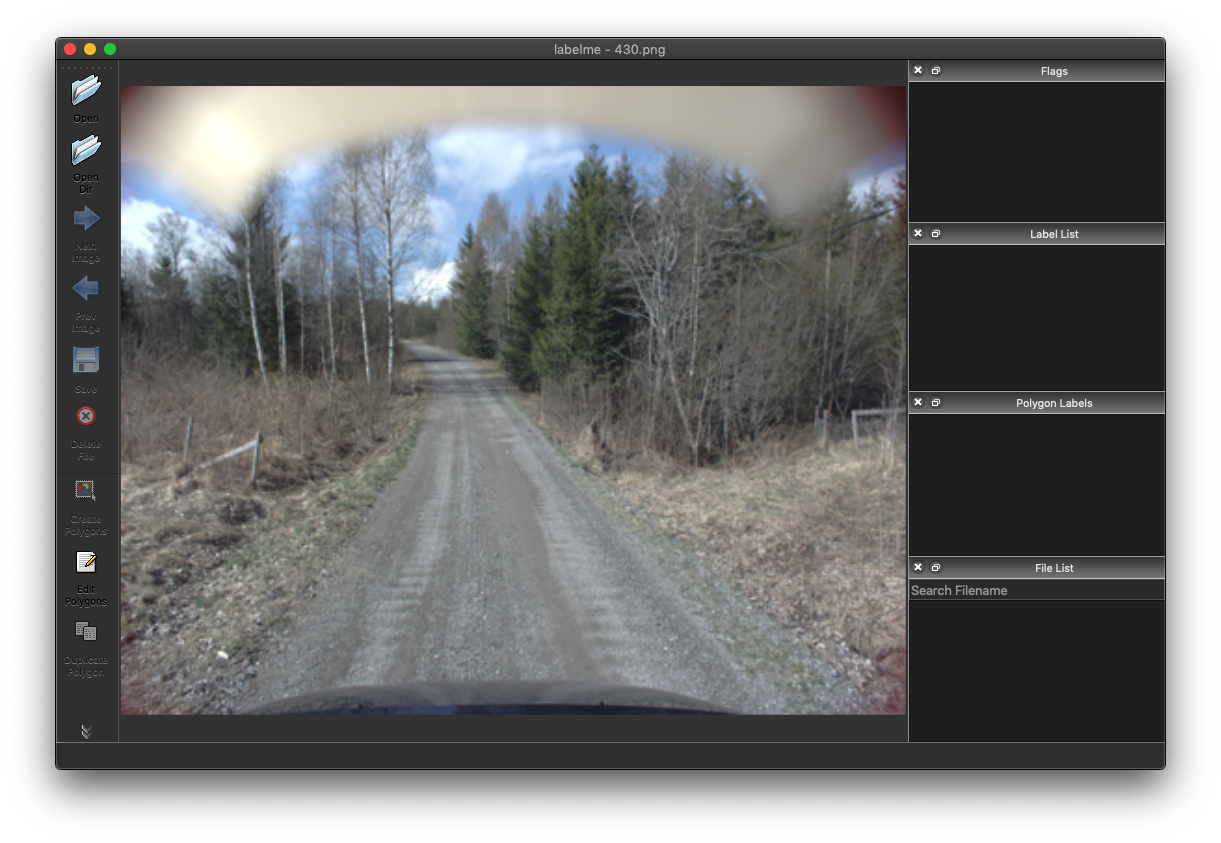
\includegraphics[width=.75\linewidth]{bilder/labelme_gui.png}
\captionof{figure}{The \ac{gui} for labelme}
\label{fig:gui}
\end{subfigure}
\hspace*{\fill} % separation between the subfigures
\begin{subfigure}{.6\textwidth}
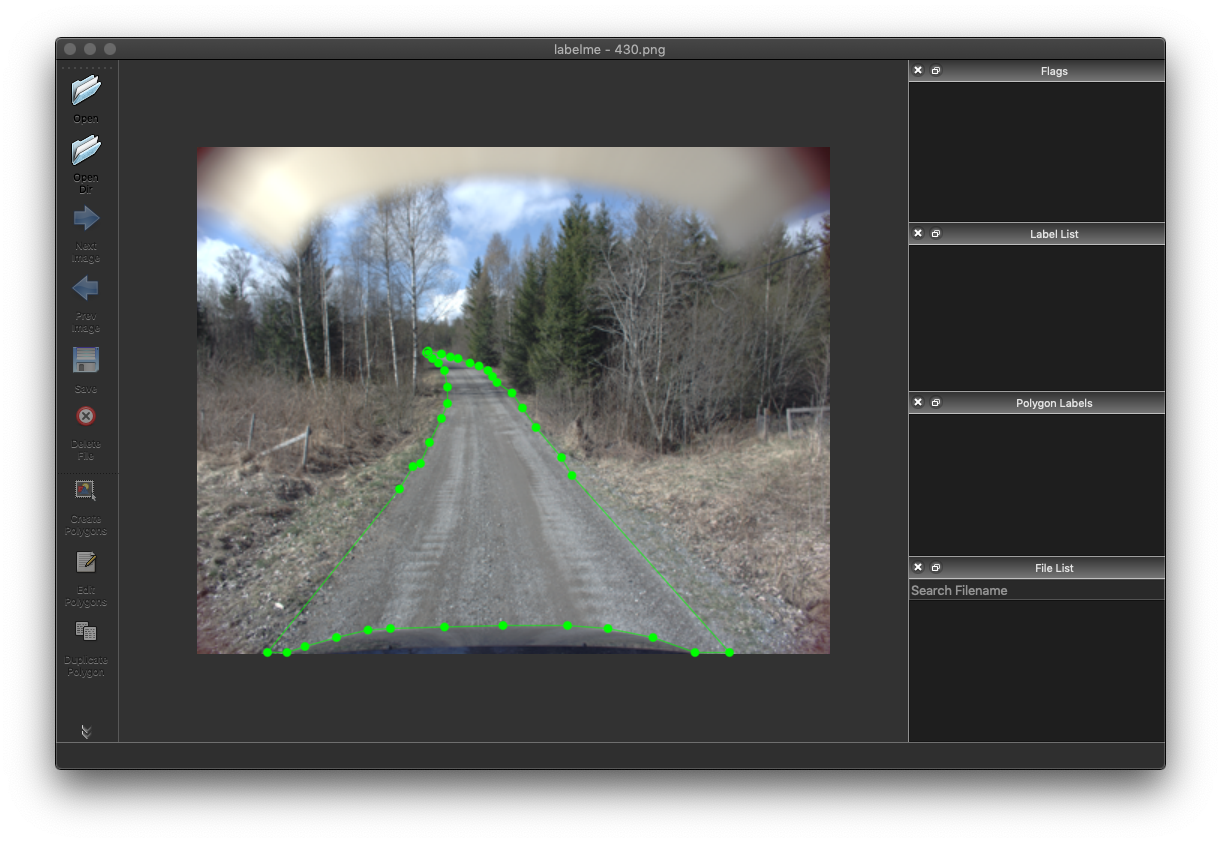
\includegraphics[width=.75\linewidth]{bilder/annotating.png}
\captionof{figure}{Drawing a polygon}
\label{fig:polygon}
\end{subfigure}
\caption{The labelme \ac{gui}}
\end{figure}

\begin{figure}[ht]
\begin{subfigure}{.6\textwidth}
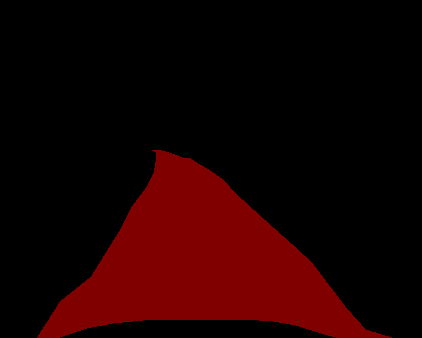
\includegraphics[width=.6\linewidth]{bilder/label_method.png}
\captionof{figure}{}
\label{fig:gt_method}
\end{subfigure}
\hspace*{\fill} % separation between the subfigures
\begin{subfigure}{.6\textwidth}
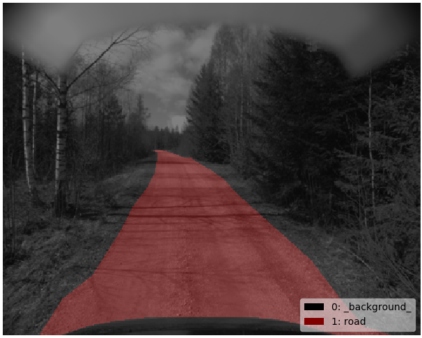
\includegraphics[width=.6\linewidth]{bilder/label_viz_method.png}
\captionof{figure}{}
\label{fig:superimposed_method}
\end{subfigure}
\caption{The ground truth in its original form in \cref{fig:gt_method}, and superimposed into original image in \cref{fig:superimposed_method}}
\end{figure}

The finished ground truth image consists of two classes. Where class 0 is assigned to the background, and class 1 to the road. The program \textit{labelme} was chosen due to its quick setup, its possibility to annotate data offline, and a clean \ac{gui} making it easy to draw polygons. 
 
\subsection{Keras}
\textit{Keras} is a user-friendly \ac{dl} library developed in Python. It was originally made for researchers as way to do quick experimentation, with an easy to use implementation. \textit{Keras} has quickly gained popularity among its users and is one of the most popular framework in \ac{dl} projects nowadays. The main reasons for the popularity is the user-friendliness and that \textit{Keras} can run with the same code seamlessly on \ac{cpu} or \ac{gpu} \cite{Francois_Deep_learning_with_python}. Both implementations of \ac{cnn} in this thesis is done in \textit{Keras}, and became the chosen framework due to its easy implementation of networks and powerful tools.

\subsection{The sequential network}
The sequential network implemented is made as a basic \ac{fcn}. This means the network is composed without using any fully connected layers at all. The \ac{fcn} has therefore learning filters placed everywhere, even in the decision making layers at the end of the network. This will save computation time and reduce the number of parameters compared to using fully connected dense layers.

\begin{minted}[bgcolor=LightGray, linenos, fontsize=\footnotesize]{python}
# Initializing
model = models.Sequential()

# Input layer
model.add(layers.Conv2D(16, 5, strides=(2, 2), padding='same', activation='relu', 
input_shape=input_shape))

# Conv layers
model.add(layers.Conv2D(16, 5, strides=(2, 2), padding='same', activation='relu'))
model.add(layers.Conv2D(32, 5, strides=(2, 2), padding='same', activation='relu'))
model.add(layers.Conv2D(32, 5, strides=(2, 2), padding='same', activation='relu'))
model.add(layers.Conv2DTranspose(32, 5, strides=(2, 2), padding='same', 
activation='relu'))
model.add(layers.Conv2DTranspose(32, 5, strides=(2, 2), padding='same', 
activation='relu'))
model.add(layers.Conv2DTranspose(16, 5, strides=(2, 2), padding='same', 
activation='relu'))
model.add(layers.Conv2DTranspose(16, 5, strides=(2, 2), padding='same', 
activation='relu'))

# Output layer
model.add(layers.Conv2D(1, 1, strides=(1, 1), padding='same', activation='sigmoid'))

# Prints the network structure summary
model.summary()
# Adding loss and optimizer
model.compile(loss='binary_crossentropy', optimizer='adam', metrics=['acc'])
\end{minted}

As seen in the code snippet above, this is the implementation of the sequential network used in the thesis. The input tensor (which is (224x224x3)) goes from the input layer through each layer until the output layer is reached. 
There is both a downsampling- and an upsampling-process in the network. In the downsampling-process consisting of four downsampling layers, the height and width is reduced from (224x224) to (14x14). Each step in the following list represents a layers downsampling and has the depth included:
\begin{itemize}
    \item \textit{(112x112x16)}
    \item \textit{(56x56x16)}
    \item \textit{(28x28x32)}
    \item \textit{(14x14x32)}
\end{itemize}
Then the upsampling process also with four layers continues sampling from (14x14) to (224x224) in the height- and width-size of the tensor. Every step in the list represents a layers upsampling and the depth is included here as well:
\begin{itemize}
    \item \textit{(28x28x32)}
    \item \textit{(56x56x32)}
    \item \textit{(112x112x16)}
    \item \textit{(224x224x16)}
\end{itemize}
The last layer is the output layer containing sigmoid activation. It has the shape (224x224x1).

The sequential network is included as the baseline in the thesis. It is done in order to benchmark it against the state-of-the-art implementation of the residual network (U-Net). In that way it will be possible to compare the differences between a basic sequential- and a state-of-the-art residual-network, trained on the same data.
\subsubsection{Loss}
There are simple guidelines which can be used for choosing the right loss. If there is a two-class classification problem, a loss called \textit{"binary\_crossentropy"} will be a natural choice \cite{Francois_Deep_learning_with_python}. This is therefore the loss used in the sequential network, and it is described mathematically in the \cref{eq:binary_cross_entropy}.

\begin{equation}\label{eq:binary_cross_entropy}
\begin{aligned}
L_{BCE} = -\sum_{i=1}^{C=2}t_{i} log (f(s_{i})) = -t_{1} log(f(s_{1})) - (1 - t_{1}) log(1 - f(s_{1}))
\end{aligned}
\end{equation}

\begin{equation}\label{eq:sigmoid_function_4}
\begin{aligned}
f(s_i)= \frac{1}{1 + e^{s_i}}
\end{aligned}
\end{equation}

Where $BCE$ is short for binary cross entropy. $C_i$ is the classes, $t_i$ and $s_i$ is the target and the score respectively. The score goes first through an sigmoid activation described in \cref{eq:sigmoid_function_4}, before the loss is further computed with a cross-entropy loss.

\subsection{The residual network}
The residual network in this thesis is loosely based on the state-of-the-art U-Net, which is further described in the paper \cite{RFB15a_u-net}. The actual implementation is as stated in the code, based on a tutorial from Kjetil Åmdal-Sævik \cite{website:u-net_implementation}, and is illustrated in the following code snippet. 

\begin{minted}[bgcolor=LightGray, linenos, fontsize=\footnotesize]{python}
# U-Net model
# The implementation is based on: 
# "https://www.kaggle.com/keegil/keras-u-net-starter-lb-0-277"

inputs = Input((int(config['data_processing']['x_pic']), 
int(config['data_processing']['y_pic']), 3))

# Layers
conv_1 = Conv2D(16, (3, 3), activation='relu', kernel_initializer='he_normal', 
padding='same')(inputs)
conv_1 = Dropout(0.1)(conv_1)
conv_1 = Conv2D(16, (3, 3), activation='relu', kernel_initializer='he_normal', 
padding='same')(conv_1)
pool_1 = MaxPooling2D((2, 2))(conv_1)
conv_2 = Conv2D(32, (3, 3), activation='relu', kernel_initializer='he_normal', 
padding='same')(pool_1)
conv_2 = Dropout(0.1)(conv_2)
conv_2 = Conv2D(32, (3, 3), activation='relu', kernel_initializer='he_normal',
padding='same')(conv_2)
pool_2 = MaxPooling2D((2, 2))(conv_2)

conv_3 = Conv2D(64, (3, 3), activation='relu', kernel_initializer='he_normal', 
padding='same')(pool_2)
conv_3 = Dropout(0.2)(conv_3)
conv_3 = Conv2D(64, (3, 3), activation='relu', kernel_initializer='he_normal', 
padding='same')(conv_3)
pool_3 = MaxPooling2D((2, 2))(conv_3)

conv_4 = Conv2D(128, (3, 3), activation='relu', kernel_initializer='he_normal', 
padding='same')(pool_3)
conv_4 = Dropout(0.2)(conv_4)
conv_4 = Conv2D(128, (3, 3), activation='relu', kernel_initializer='he_normal', 
padding='same')(conv_4)
pool_4 = MaxPooling2D(pool_size=(2, 2))(conv_4)

conv_5 = Conv2D(256, (3, 3), activation='relu', kernel_initializer='he_normal', 
padding='same')(pool_4)
conv_5 = Dropout(0.3)(conv_5)
conv_5 = Conv2D(256, (3, 3), activation='relu', kernel_initializer='he_normal', 
padding='same')(conv_5)

up_6 = Conv2DTranspose(128, (2, 2), strides=(2, 2), padding='same')(conv_5)
up_6 = concatenate([up_6, conv_4])
conv_6 = Conv2D(128, (3, 3), activation='relu', kernel_initializer='he_normal', 
padding='same')(up_6)
conv_6 = Dropout(0.2)(conv_6)
conv_6 = Conv2D(128, (3, 3), activation='relu', kernel_initializer='he_normal', 
padding='same')(conv_6)

up_7 = Conv2DTranspose(64, (2, 2), strides=(2, 2), padding='same') (conv_6)
up_7 = concatenate([up_7, conv_3])
conv_7 = Conv2D(64, (3, 3), activation='relu', kernel_initializer='he_normal', 
padding='same')(up_7)
conv_7 = Dropout(0.2)(conv_7)
conv_7 = Conv2D(64, (3, 3), activation='relu', kernel_initializer='he_normal', 
padding='same')(conv_7)

up_8 = Conv2DTranspose(32, (2, 2), strides=(2, 2), padding='same')(conv_7)
up_8 = concatenate([up_8, conv_2])
conv_8 = Conv2D(32, (3, 3), activation='relu', kernel_initializer='he_normal', 
padding='same')(up_8)
conv_8 = Dropout(0.1)(conv_8)
conv_8 = Conv2D(32, (3, 3), activation='relu', kernel_initializer='he_normal', 
padding='same')(conv_8)

up_9 = Conv2DTranspose(16, (2, 2), strides=(2, 2), padding='same')(conv_8)
up_9 = concatenate([up_9, conv_1], axis=3)
conv_9 = Conv2D(16, (3, 3), activation='relu', kernel_initializer='he_normal', 
padding='same')(up_9)
conv_9 = Dropout(0.1)(conv_9)
conv_9 = Conv2D(16, (3, 3), activation='relu', kernel_initializer='he_normal', 
padding='same')(conv_9)

outputs = Conv2D(1, (1, 1), activation='sigmoid')(conv_9)

model = Model(inputs=[inputs], outputs=[outputs])
model.compile(optimizer='adam', loss='binary_crossentropy', metrics=['accuracy'])
model.summary()

\end{minted}

The U-Net with its skipping connection features is already briefly described in the related work section. When implementing the network, the choice of loss and optimizer are set to be the same as for the sequential network. The implementation in this thesis loosely based on the U-Net will further be referenced to as the residual network.

\begin{figure}[ht]
    \centering
    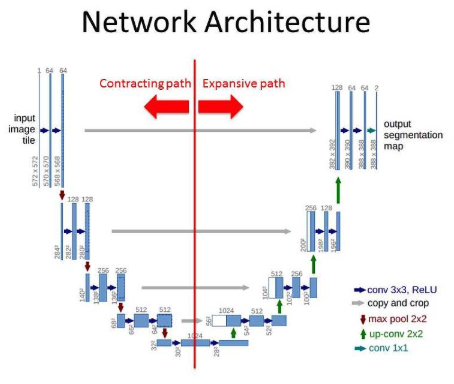
\includegraphics[width=0.8\textwidth]{bilder/u-net_architecture_method.png}
    \caption{The U-Net architecture illustrated with skip connections \cite{website:u-net_method}}
    \label{fig:u_net_method_chapter}
\end{figure}

When testing the performance in the residual network, it proved to be able to provide quite accurate predictions from few training samples. Gaining accurate predictions with few training images are the main priorities when implementing the network architecture. Having it successfully implemented will save a lot of time because it is sufficient to only manually annotate a few images. To have accurate predictions means the network performs well, and can be able to provide better results in the form of good predictions. 

\begin{figure}[ht]
    \centering
    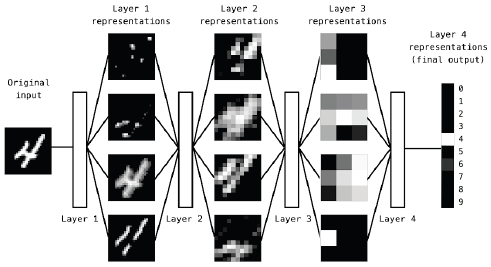
\includegraphics[width=0.8\textwidth]{bilder/layers_features.png}
    \caption{The features extracted from different layers in \ac{cnn} \cite{Francois_Deep_learning_with_python}}
    \label{fig:layers_features}
\end{figure}

An important difference between the sequential and the residual network, its the residual networks capability to provide skipping connections. These skipping connections transfers information from each downsampling layer, directly to its upsampling layer respectively, as illustrated with the gray arrows in \cref{fig:u_net_method_chapter}. The upsampling layers concatenates its existing information with the information from the skipping connections. As seen in \cref{fig:layers_features}, each layer in a \ac{cnn} extracts different types of features. When the U-Net architecture concatenates the local information provided from the skipping connections, with the global information from the upsampling layers; this results in an improved and efficient feature extraction.  

\subsection{Transfer learning}
Before the transfer learning can start, the network needs to train on a dataset and save the weights respectively. This is done by training on the \textit{Freiburg Forest} dataset \cite{freiburg_dataset_valada16iser}. The \textit{Freiburg Forest} dataset is developed in the University of Freiburg in Germany. It consists of images from off-road environments taken from the Black Forest area in Schwarzwald. The reason why this dataset is such a interesting choice to use, is its similarities to the custom made datasets used in this thesis. The custom made datasets does also have images from an off-road scene.

When the training is finished the weights are saved and the fine-tuning can begin after one last step. The last step is to change the training set to the original dataset used in this thesis.

\begin{minted}[bgcolor=LightGray, linenos, fontsize=\footnotesize]{python}
# Transfer learning
if config['train/test/debug'].getboolean('transfer') is True:
model_res = load_model('models/freiburg/weights.45-0.99.hdf5')
for layer in model_res.layers[:32]:
layer.trainable = False 

# Train model
model_res.fit(x_train, y_train, batch_size=10,
epochs=int(config['train/test/debug']['epochs']),
shuffle=True, validation_data=(x_val, y_val),
callbacks=callbacks_model_res)
\end{minted}
\todo{Oppdater koden til nåværende status, og skriv om til fryste vektverdier fra begge nett}
As seen in the code snippet above, the model retrieves the saved weights from the training with the \textit{Freiburg Forest} dataset in line three. From there it freezes all the layers up to layer 32, which means when the training starts again the weights from those layers will not change. Then the network starts training with the original dataset in line eight. Since all the layers up to layer 32 are frozen, only the last layer will change its weights during this training. This is called fine-tuning. 

\subsection{Tensorboard}
A handy way to gain control over the training, in order to tweak parameters and control the models accuracy, is to use Tensorboard. Tensorboard is a visual tool developed by TensorFlow providing full overview of the training, while training. It is easy to set up in the terminal.
\begin{figure}[ht]
    \centering
    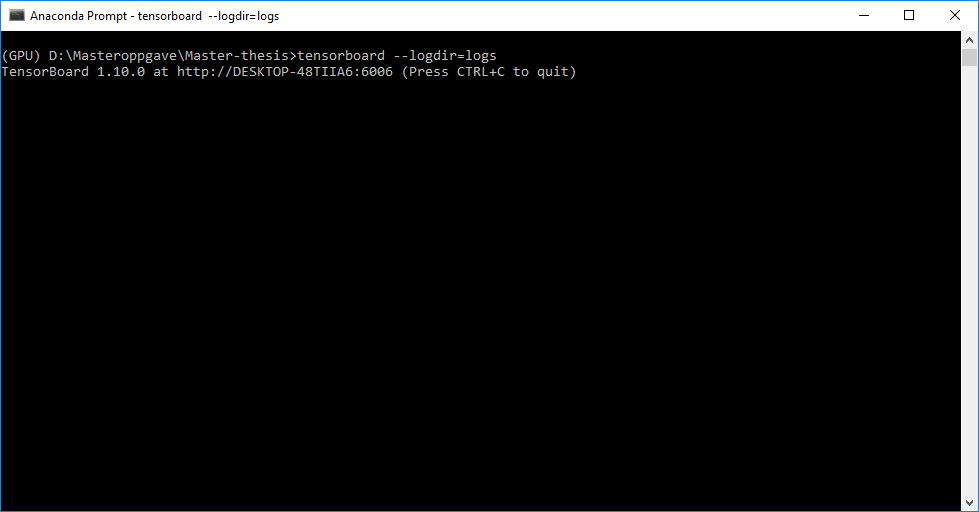
\includegraphics[width=0.8\textwidth]{bilder/tensorboard_anaconda_prompt.PNG}
    \caption{Initializing Tensorboard from terminal}
    \label{fig:tensorboard_anaconda_prompt}
\end{figure}
As illustrated in \cref{fig:tensorboard_anaconda_prompt} Tensorboard is up and running with the following command: 

\begin{minted}[bgcolor=LightGray, linenos, fontsize=\footnotesize]{bash}
tensorboard --logdir=<log> 
\end{minted}
Where all you need to enter is the address to the log folder the algorithm provides. 
\newline
When using Tensorboard with \textit{Keras}, it is necessary to use \textit{callbacks} in the code. As stated by the \textit{Keras} documentation on their website:
\newline
\newline
\textit{"A callback is a set of functions to be applied at given stages of the training procedure. You can use callbacks to get a view on internal states and statistics of the model during training. You can pass a list of callbacks (as the keyword argument callbacks) to the .fit() method of the Sequential or Model classes. The relevant methods of the callbacks will then be called at each stage of the training."}\cite{website:Keras_doc}. 
\newline
\newline
Using callbacks it is possible to decide which information/process to include and when it should be executed during the training process.

\begin{figure}[ht]
\centering
\begin{subfigure}[b]{\textwidth}
\centering
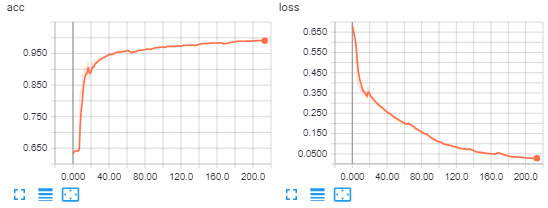
\includegraphics[width=1\textwidth]{bilder/tensorboard_acc.png}
\caption{Training accuracy and loss}
\end{subfigure}
\hfill
\begin{subfigure}[b]{\textwidth}
\centering
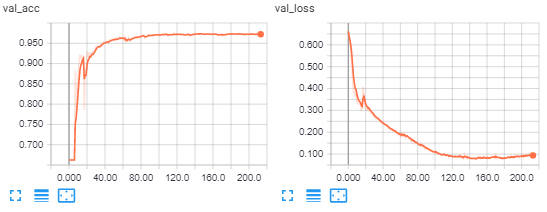
\includegraphics[width=1\textwidth]{bilder/tensorboard_val_acc.png}
\caption{Validation accuracy and loss}
\end{subfigure}
\caption{Accuracy and loss for both training and validation visualized in Tensorboard}
\label{fig:accuracy_loss}
\end{figure}
Two standard graphs used to check the quality of the \ac{dl} model is \textit{"accuracy"} and \textit{"loss"}, which are found under the tab \textit{"SCALARS"}. 
\begin{figure}[ht]
    \centering
    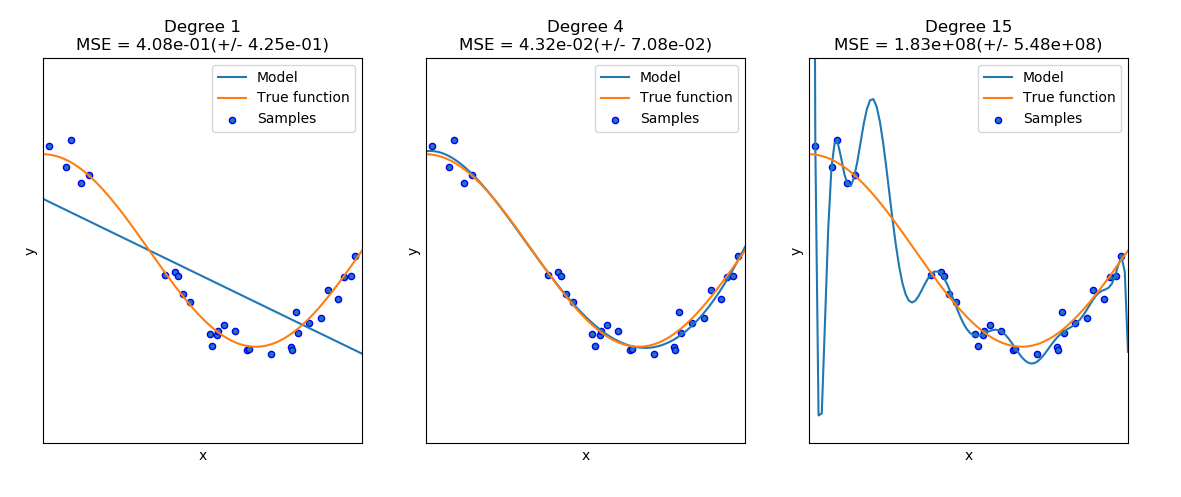
\includegraphics[width=1\textwidth]{bilder/overfitting_underfitting.png}
    \caption{Underfitting, perfect sampling and overfitting \cite{website:overfitting_underfitting}}
    \label{fig:overfitting_underfitting}
\end{figure}
To have the opportunity to visualize these graphs during training, is an advantage. This is due to the possibility of easily spotting errors like \textit{overfitting} or \textit{underfitting}, and if the accuracy in the model is fulfilling user expectations. Examples of \textit{underfitting} from the left image, perfect sampling in the middle and overfitting in the right image, can be seen in \cref{fig:overfitting_underfitting}. As seen in \cref{fig:accuracy_loss} the accuracy and loss in both training and validation fulfil expectations. 
By observing that the loss function steadily decreases into a smooth curve indicates that there is neither \textit{overfitting} nor \textit{underfitting} in the model.

\begin{figure}[ht]
\centering
\begin{subfigure}[b]{\textwidth}
\centering
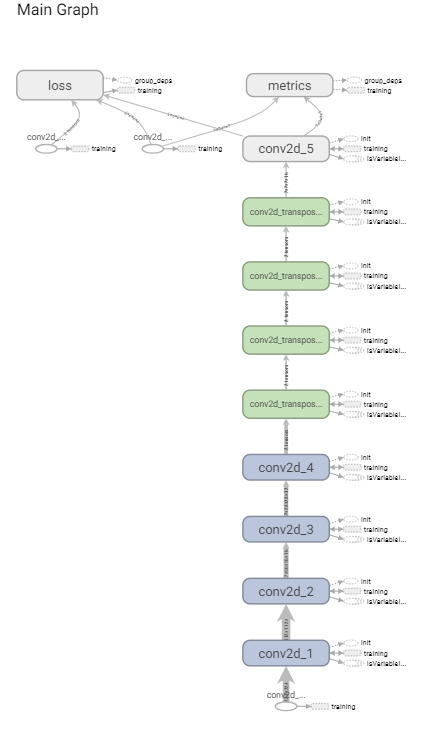
\includegraphics[width=0.5\textwidth]{bilder/tensorboard_graph_1.PNG}
\caption{Main graph}
\end{subfigure}
\hfill
\begin{subfigure}[b]{\textwidth}
\centering
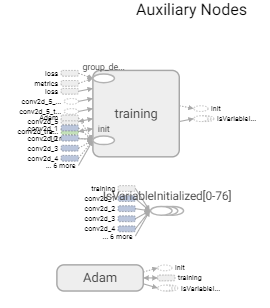
\includegraphics[width=0.5\textwidth]{bilder/tensorboard_graph_2.PNG}
\caption{Auxiliary nodes}
\end{subfigure}
\caption{The sequential network architecture visualized in Tensorboard}
\label{fig:graph}
\end{figure}

Another tab in Tensorboard called \textit{"GRAPHS"} shows the current networks architecture. Being able to see all the layers, optimizer function and connections, helps the user see the whole network in a visualized perspective. There is possible to rename each layer in the model according to the user's own preference. 
\section{Predictions}
A prediction in this context is when the networks in this thesis produce a qualified guess of what value each pixel in the image shall be assigned, from either one of the two classes. This is the basis for what will become the automatically annotated images. After the network has updated its internal state satisfactorily, the training can stop, and it is ready to be fed new images it has never seen before. The network will then predict an output given the input of the new data, which will use the finished trained internal state of the network to predict. The predictions with sufficiently good results will in the end become the automatically annotated images this thesis tries to produce. When all the predictions are made, they will in the most cases contain some adverse features like different types of noise or choppy edges in the classification. To avoid these types of artifacts several techniques from computer vision can be applied.

\subsection{Thresholding}
The first tool used is called thresholding. It removed the predicted pixels in the image which has a value below the given threshold. When the networks predicts pixel values, this happens in the range between 0-1. The thresholding will convert that fuzzy logic to values which are either 0 or 1. Where class 0 is background and class 1 is road.
\begin{minted}[bgcolor=LightGray, linenos, fontsize=\footnotesize]{python}
# Filter out values with less certainty than 65 %
prediction = np.where(prediction > 0.65, np.ones_like(prediction), 
np.zeros_like(prediction))
\end{minted}

\begin{equation}\label{eq:thresholding}
\begin{aligned}
{f(x_i)=
\begin{cases}
    1 & \text{ $x_i$ > 0.65 }  \\
    0 & \text{ $x_i$ $\leq$ 0.65 }
\end{cases}}
\end{aligned}
\end{equation}

What the code snippet above does, is to filter all values where $x_i$ are the predicted values, and assign them to either 0 or 1. All values over 0.65 are assigned to 1 and all values up to 0.65 are assigned to 0. This is described in \cref{eq:thresholding}. The thresholding will therefore remove some noise and assign values up to the threshold as background instead of road.

\subsection{Morphological operations}
\todo{Legg til en paragraf med morfologiske operasjoner}
\subsection{Connected component analysis}
The next operation used in order to remove larger sections of noise predicted in the image is called connected component analysis. When implemented in this thesis it removes all sections in the images which contains less than 5000 pixels. This means in the most cases that all of the remaining noise in the image will be removed. The connected component analysis has one disadvantage which is when the road predicted is less than the threshold value of 5000 pixels. Then the whole prediction will consists of only background. This only happens in a very limited amount of the images. The reason for setting the pixel threshold to 5000 became clear after testing different values. Lower values did not remove all the noise in the image, while much larger values could remove the correct predicted road. 
\subsection{Binary hole filling}
The last computer vision technique used in this thesis is to fill all the holes in the remaining predicted road. That operation is simply done by the following line of code:
\begin{minted}[bgcolor=LightGray, linenos, fontsize=\footnotesize]{python}
predictions = scipy.ndimage.morphology.binary_fill_holes(predictions)
\end{minted}

The operation is described in the Scipy-documentation and reads as follows:
\newline
\newline
\textit{"The algorithm used in this function consists in invading the complementary of the shapes in input from the outer boundary of the image, using binary dilations. Holes are not connected to the boundary and are therefore not invaded. The result is the complementary subset of the invaded region." \cite{website:scipy}.} 

\section{Experiments}
This last part of the method chapter will cover the experiments done in this thesis. In the form of describing the structure of the datasets, and the choices made regarding choosing the number of images in the train-, test- and validation sets. Further this last part of the section will go through the training configurations chosen during training.  
\subsection{Datasets}\label{datasets}
This thesis uses three datasets. Two of them contains only raw images, while one of them has existing ground truth. The one with existing ground truth is the \textit{Freiburg Forest} dataset briefly described above. This is a public dataset, and suits this thesis due to its off-road environment. As described in their website:
\newline
\newline
\textit{"The Freiburg Forest dataset was collected using our Viona autonomous mobile robot platform equipped with cameras for capturing multi-spectral and multi-modal images. The dataset may be used for evaluation of different perception algorithms for segmentation, detection, classification, etc. All scenes were recorded at 20 Hz with a camera resolution of 1024x768 pixels. The data was collected on three different days to have enough variability in lighting conditions as shadows and sun angles play a crucial role in the quality of acquired images. The robot traversed about 4.7 km each day. We provide manually annotated pixel-wise ground truth segmentation masks for 6 classes: Obstacle, Trail, Sky, Grass, Vegetation, and Void."} \cite{website:deepscene_freiburg_forest_website}. 
\newline
\newline
As described in the website, the dataset consists of six classes. Since this thesis wants to investigate a two class problem containing road and background, the classes other than road will be masked as background.

\begin{table}[ht]
\centering
\begin{tabular}{lllll}
\hline
\textbf{Dataset} & \textbf{Training-}  & \textbf{Testing-}  & \textbf{Validation-images} \\ \hline
Freiburg Forest dataset & \quad 207  & \quad 136  & \quad 23   \\ 
Custom 1 dataset  & \quad 40  & \quad 394  & \quad 5   \\
Custom 2 dataset  & \quad 147  & \quad 1472 + 404  & \quad 17    \\\hline
\end{tabular}
\caption{Dataset structures}
\label{table:dataset}
\end{table}
The second dataset is named \textit{Custom 1}, and the last is titled \textit{Custom 2}. As earlier stated these are two datasets originally consisting of only raw images without ground truth. This thesis wants to investigate if there is an opportunity to automatically predict the annotations to these images given only a few manually annotated images. The task of manually annotate lots of pictures is both time-consuming and repetitive, and having this task automated by a network would be an advantage. The few images which are manually annotated in these two datasets are the ones in the training and validation sets respectively. The dataset structure is illustrated in \cref{table:dataset}. In the table, it is possible to see explicitly the number of images in each directory. One can notice the amount of training images is significantly higher than in both the custom made datasets. This means there is a higher probability that the \textit{Freiburg Forest} dataset will provide a more generalized network than any of the two custom made datasets, even though the residual network is known to provide good results with few training samples \cite{website:u_net_article}. As discussed earlier, this thesis investigates the possibility of retrieving many automatically annotations from few training samples. The experimentation will consist of using the more generalized features gained from the \textit{Freiburg Forest} dataset combined with the residual network implementation. This is done in order to hopefully retrieve a certain percentage of automatically generated annotations, with decent accuracy. The process is partly described above in the transfer learning section in this chapter.

\begin{figure}[ht]
\minipage{0.32\textwidth}
  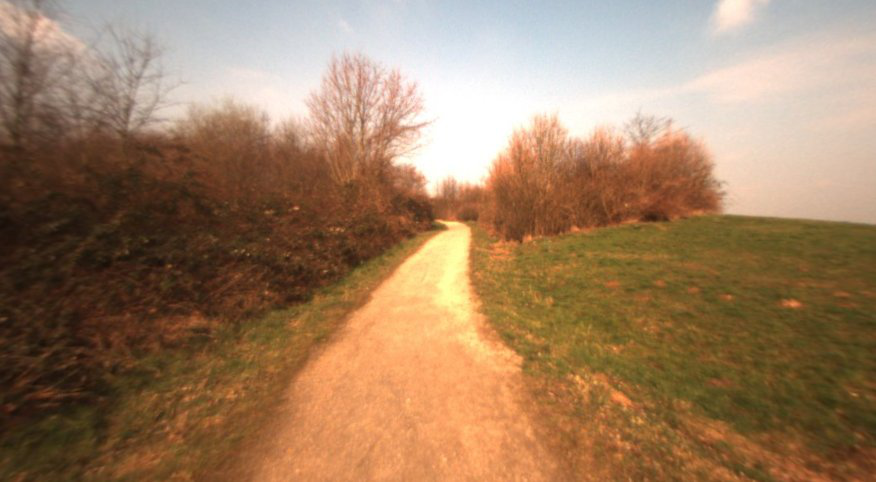
\includegraphics[width=\linewidth, height=3.5cm]{bilder/freiburg.png}
  \caption{An image from the \textit{Freiburg Forest} dataset}\label{fig:awesome_image1}
\endminipage\hfill
\minipage{0.32\textwidth}
  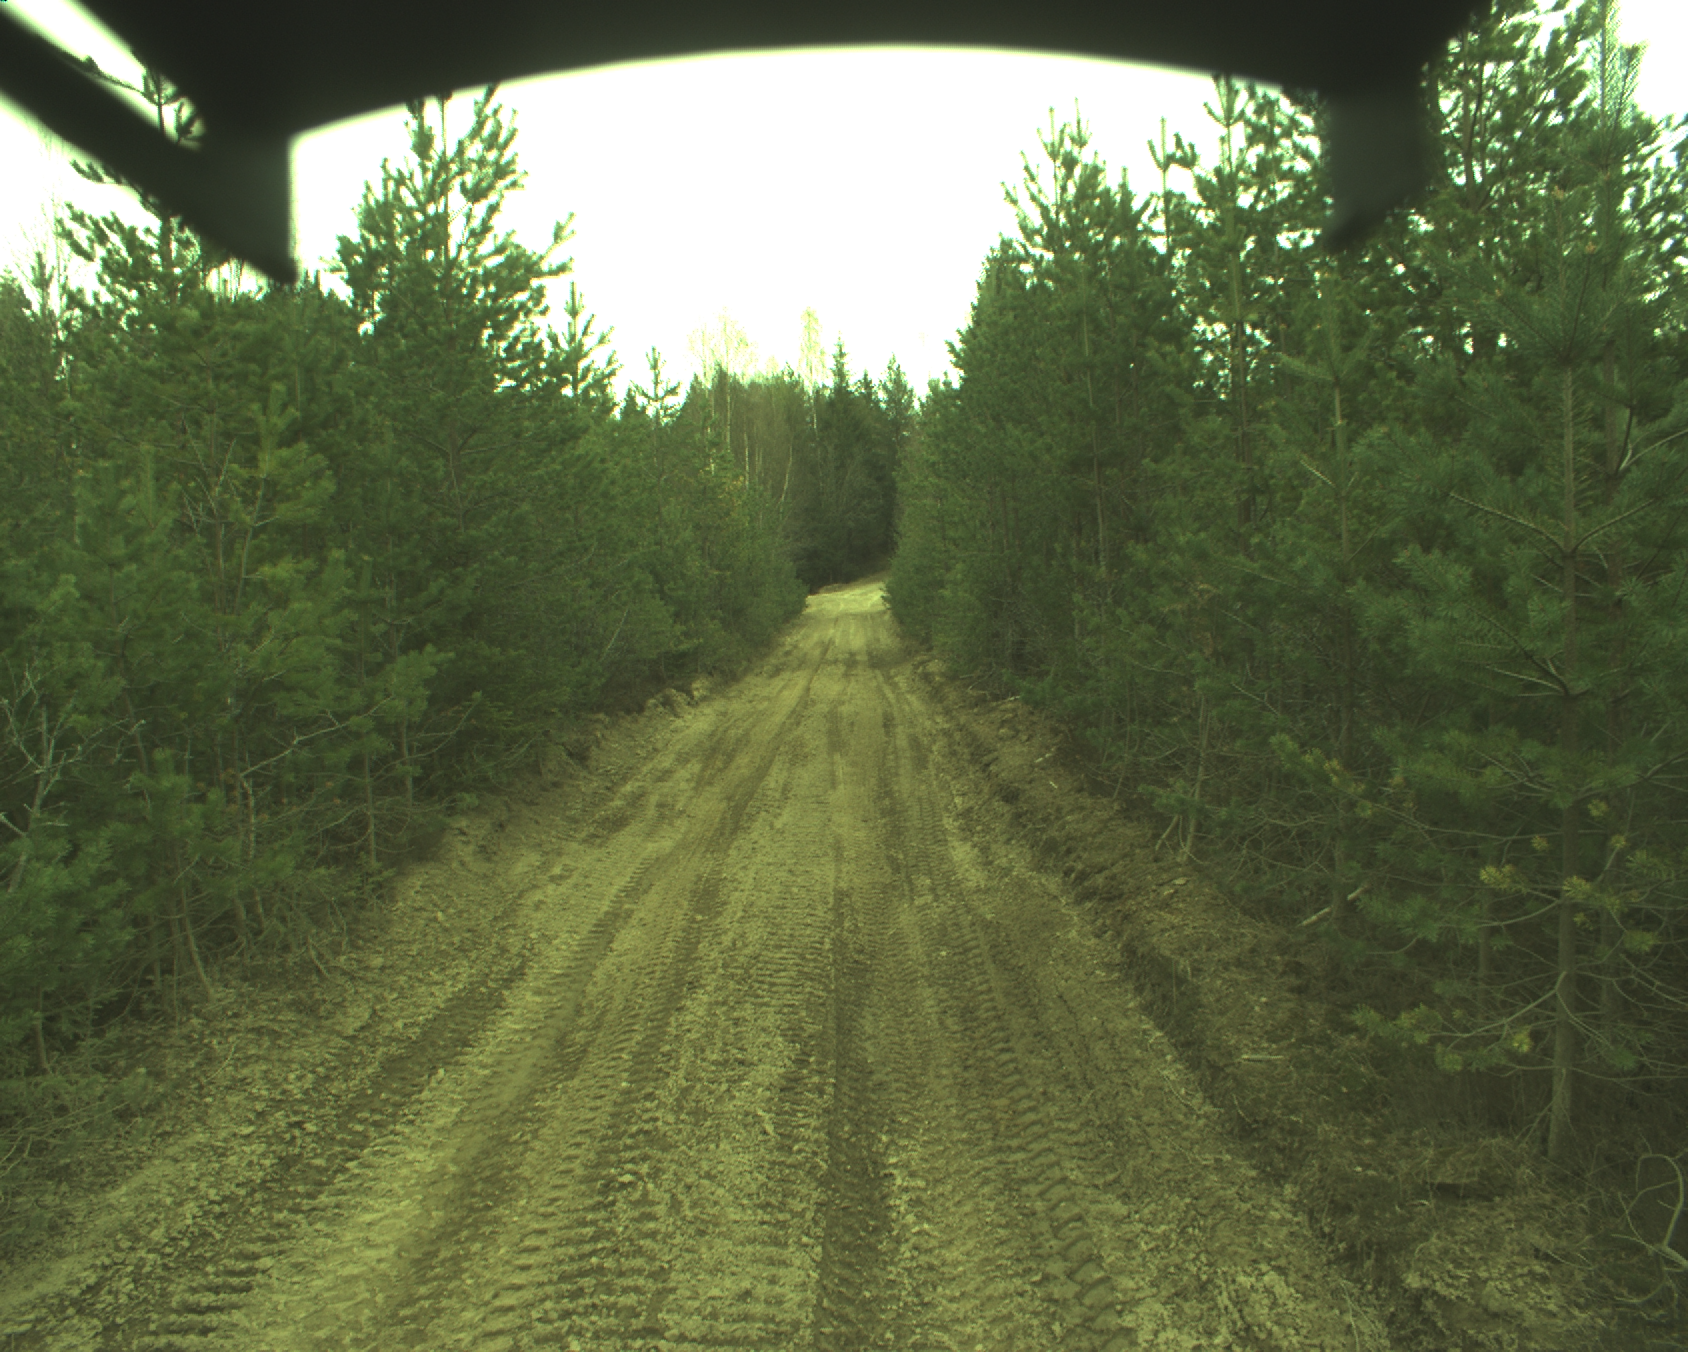
\includegraphics[width=\linewidth, height=3.5cm]{bilder/custom_1.png}
  \caption{An image from the \textit{Custom 1} dataset}\label{fig:awesome_image2}
\endminipage\hfill
\minipage{0.32\textwidth}%
  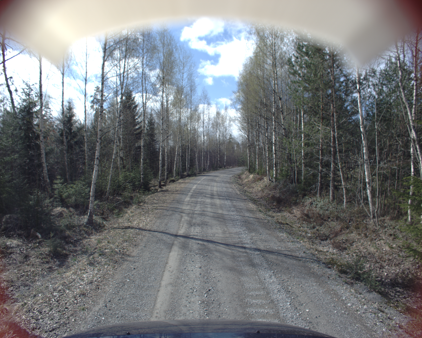
\includegraphics[width=\linewidth, height=3.5cm]{bilder/custom_2.png}
  \caption{An image from the \textit{Custom 2} dataset}\label{fig:awesome_image3}
\endminipage
\end{figure}

To get a visual understanding of which type of scene is included in each dataset an example image from each dataset is provided in \cref{fig:awesome_image1}, \cref{fig:awesome_image2}, and \cref{fig:awesome_image2}. It is possible to see some similarities between all datasets, hence understand why the \textit{Freiburg Forest} dataset is used as the dataset for the transfer learning. The \textit{Custom 1} dataset is an off-road dataset contains 439 images. The scene consists of similar images like the one illustrated in \cref{fig:awesome_image2}. The 45 manually annotated training- and validation images are chosen as every tenth image ranging from start to end in the dataset. This means that small fractions from the full sequence may be included in the training set. This way of choosing training images is not a normal method in \ac{dl}, but is used since the goal of this thesis is to mostly predict highly correlated data. The cost of choosing training data like this may reduce some of the network's generalization capability. The hypothesis is that since the data is very correlated, the network will still be able to predict the test images with satisfactorily high accuracy. 

The last dataset used in the thesis is \textit{Custom 2}. This dataset consists of 2040 images in total. It contains 164 manually annotated training- and validation images that are chosen every tenth image ranging from start until number 1636 in the dataset. An example image from \textit{Custom 2} is illustrated in \cref{fig:awesome_image3}. The difference from \textit{Custom 1} apart from having a slightly different type of scene, consists of a second test set containing 404 images. This test set is taken from the last sequence in the dataset and nothing of its sequence has been included in either the training or the validation set. This is done in order to check if the network is able to generalize well on completely new unseen data, which in theory should be completely uncorrelated from the images in the training set.

The datasets need to be structured in order to gain control over which data to use when training, or when testing. The structure used in this thesis is illustrated in \cref{fig:dataset_structure}. This structure is equal for all three datasets with one exception. The \textit{Freiburg Forest} dataset does also include ground truth images for the test set.

\begin{figure}[ht]
    \centering
    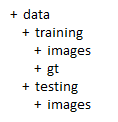
\includegraphics[width=0.4\textwidth]{bilder/dataset_structure.PNG}
    \caption{This thesis dataset structure}
    \label{fig:dataset_structure}
\end{figure}

Note that from both custom made datasets, the only images containing ground truth are the training images. Optimally all the images included in these datasets would have ground truth. In that way, the algorithm can be able to measure accuracy and loss in predictions both during training and testing. The reason why the ground truth only are included in the training set for both custom datasets is as earlier described due to the high cost of manually labeling an image. To check how good the predictions provided by the network are, this can only be done visually by comparing the road predictions to where the road actually is in the original image.

The training directory is further split into following list variables:
\begin{itemize}
    \item \textit{x\_train}
    \item \textit{y\_train}
    \item \textit{x\_val}
    \item \textit{y\_val}
\end{itemize}
Where \textit{x\_train} and \textit{y\_train} refers to the training images and its ground truth's respectively. \textit{x\_val} refers to validation images, and \textit{y\_val} is the ground truth's for the validation images. The network will only train on the training set, then check accuracy on the validate set and predict values on the testing set. The validation and test set should on a general basis be data that the network never has seen before. As described in the section above, only a few of the images were manually annotated. This means the dataset only has a small number of images to train on. Hence, the percentage of images split into the validation set is put to ten percent. Optimally should this number be higher, but being able to train on most available images got a higher priority in this thesis. Another reason for experimenting with a low percentage of training images is to check how many images could be automatically annotated satisfactory with as few manually annotated training images as possible.

\subsection{Training}

\begin{table}[ht]
\centering
\begin{tabular}{ll}
\hline
\textbf{Specification} & \textbf{Description} \\ \hline
\ac{cpu} & i7-6700k \\
\ac{gpu} & GeForce GTX 1070  \\
\ac{gpu}-memory & 8 GB  \\
RAM & 16 GB \\
Operating system & Windows 10  \\ \hline
\end{tabular}
\caption{System specifications}
\label{table:system_spec}
\end{table}

The computer used for the training has the following system specifications described in \cref{table:system_spec}.
When the training is executed the different runs consists of a set of common parameters which are described in \cref{table:hyperparameters}. 

\begin{table}[ht]
\centering
\begin{tabular}{ll}
\hline
\textbf{Description} & \textbf{Value/Name}  \\ \hline
Loss &  Binary cross entropy\\
Optimizer &  adam \\
Resolution & 224x224 \\
%Size of validation set & 10\%  \\
Epochs &  5000 \\ 
Batch size & 10\\
Activation function & ReLu\\
Output layer activation & Sigmoid \\ \hline
\end{tabular}
\caption{The hyperparameters used in training}
\label{table:hyperparameters}
\end{table}

All the training cycles run both the sequential and the residual network in order to compare the two different networks in the end. The first two runs are with the \textit{Freiburg Forest} dataset. After the training runs the best weights are saved as h5 files ready for transfer learning. The next step is to load the weights, and fine-tune them for both the \textit{Custom 1} and \textit{Custom 2} dataset respectively. After the fine-tuning is finished, the final weights need to be saved, and the networks are prepared for the prediction of unseen data. 

\chapter{Results}\label{result} 
This chapter will cover the results provided by the two networks implemented. Starting with the training results, before presenting the quantitative results from the \textit{Freiburg Forest} dataset, and an indication of how the quantitative results could be in the \textit{Custom 1} and \textit{Custom 2} datasets. The last part of this chapter presents the qualitative results for some predictions in the form of visual presentation of the predicted images next to the original images.

\section{Accuracy and loss results from the training}
This section will provide the accuracy and loss results from both the training- and the validation set. The presentation of these training results will be divided into three parts, covering each dataset separately. Each figure presented will show through the accuracy on the y-axis in the left graph, and loss in the right graph. The x-axis represents the number of epochs \cite{website:epoch} in all graphs.  

\begin{figure}[ht]
\centering
\begin{subfigure}[b]{\textwidth}
\centering
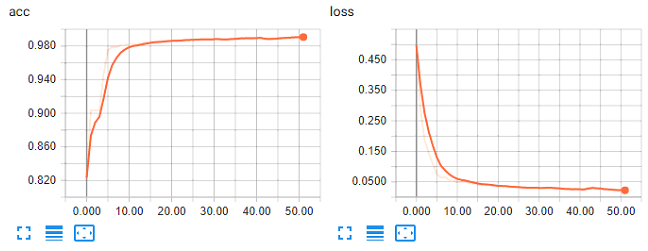
\includegraphics[width=1\textwidth]{bilder/freiburg_training/freiburg_residual_training_acc_results.png}
\caption{Training accuracy and loss}
\label{fig:freiburg_residual_acc_result}
\end{subfigure}
\hfill
\begin{subfigure}[b]{\textwidth}
\centering
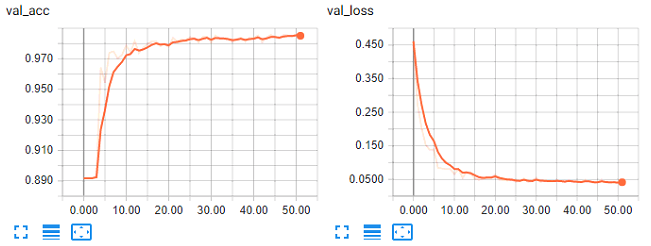
\includegraphics[width=1\textwidth]{bilder/freiburg_training/freiburg_residual_training_val_acc_results.png}
\caption{Validation accuracy and loss}
\label{fig:freiburg_residual_val_acc_result}
\end{subfigure}
\caption{The training and validation set results from the residual network, trained on the \textit{Freiburg Forest} dataset}
\label{fig:freiburg_residual_result}
\end{figure}

The two networks start training on the \textit{Freiburg Forest} dataset. As presented in \cref{table:dataset} this dataset consists of 230 images split into 207 training images and 23 validation images. The training results from the residual network are visualized in \cref{fig:freiburg_residual_result}. Where \textit{acc} (accuracy) and \textit{loss} in \cref{fig:freiburg_residual_acc_result} belongs to the training images, and \textit{val\_acc} (validation accuracy) and \textit{val\_loss} (validation loss) in the \cref{fig:freiburg_residual_val_acc_result} to the validation images. The rest of the training results is presented in the same structure. The graphs in \cref{fig:freiburg_residual_acc_result} contains a high accuracy and a low loss, which is desirable. The same can be said about the validation accuracy and the validation loss in \cref{fig:freiburg_residual_val_acc_result}, which means the training did not do any overfitting. Summarized is this a successful training for the residual network from epoch 0 to epoch 50.

\begin{figure}[ht]
\centering
\begin{subfigure}[b]{\textwidth}
\centering
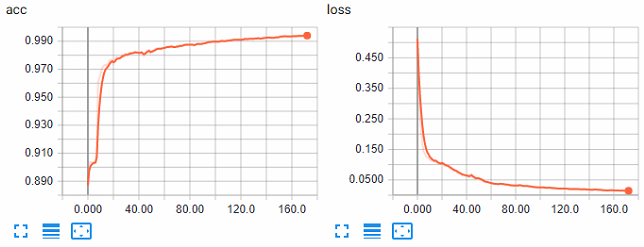
\includegraphics[width=1\textwidth]{bilder/freiburg_training/freiburg_sequential_training_acc_results.png}
\caption{Training accuracy and loss}
\label{fig:freiburg_sequential_acc_result}
\end{subfigure}
\hfill
\begin{subfigure}[b]{\textwidth}
\centering
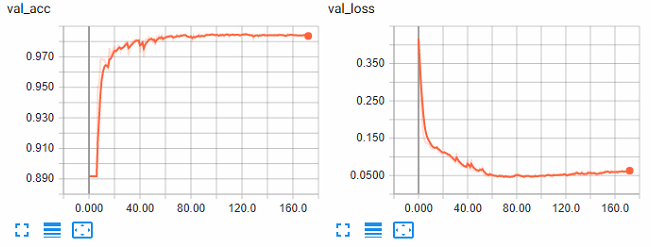
\includegraphics[width=1\textwidth]{bilder/freiburg_training/freiburg_sequential_training_val_acc_results.png}
\caption{Validation accuracy and loss}
\label{fig:freiburg_sequential_val_acc_result}
\end{subfigure}
\caption{The training and validation set results from the sequential network, trained on the \textit{Freiburg Forest} dataset}
\label{fig:freiburg_sequential_result}
\end{figure}

As illustrated in \cref{fig:freiburg_sequential_result} the sequential network follows almost the same lines as the residual networks graph, meaning this training is also considered successful. The epochs in this graph stretch from 0-160, and as seen in the validation loss around epoch 100, the curve is starting to ascent. The ascending indicates the start of possible overfitting because the training loss starts descending on approximately the same time. Therefore the training must be stopped, and the weights saved before that epoch.

\begin{figure}[ht]
\centering
\begin{subfigure}[b]{\textwidth}
\centering
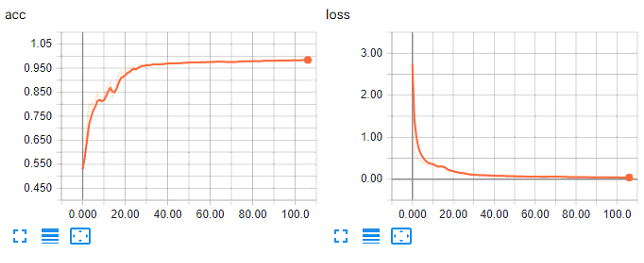
\includegraphics[width=1\textwidth]{bilder/custom_1_training/Custom_1_residual_training_acc_results.png}
\caption{Training accuracy and loss}
\label{fig:custom_1_residual_acc_result}
\end{subfigure}
\hfill
\begin{subfigure}[b]{\textwidth}
\centering
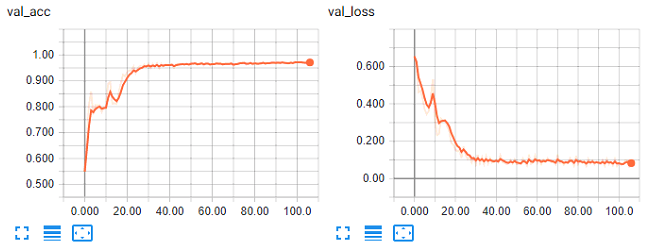
\includegraphics[width=1\textwidth]{bilder/custom_1_training/Custom_1_residual_training_val_acc_results.png}
\caption{Validation accuracy and loss}
\label{fig:custom_1_residual_val_acc_result}
\end{subfigure}
\caption{The training and validation set results from the residual network, trained on the \textit{Custom 1} dataset}
\label{fig:custom_1_residual_result}
\end{figure}

The next dataset the two networks use in their training is the \textit{Custom 1} dataset. The \cref{table:dataset} shows that this dataset consists of 40 training images, five validation images, and 394 test images. Before each training starts, the weights saved from the previous run on the \textit{Freiburg Forest} dataset are loaded into the current network. Then the most layers until the last few are frozen as described under the transfer learning section, and the network starts the training by fine-tuning the weights of the last layers. As seen in \cref{fig:custom_1_residual_acc_result} this training provides an accuracy which converges close to 100\%, and a low loss converging close to zero percent. The validation loss in \cref{fig:custom_1_residual_val_acc_result} is a little spiky, but converge around ten percent. The training loss in \cref{fig:custom_1_residual_acc_result} converge as well at approximately zero percent. In other words, this training does not look like potential overfitting. 

\begin{figure}[ht]
\centering
\begin{subfigure}[b]{\textwidth}
\centering
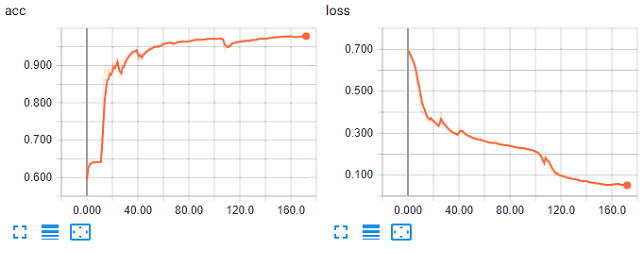
\includegraphics[width=1\textwidth]{bilder/custom_1_training/Custom_1_sequential_acc_training_results.png}
\caption{Training accuracy and loss}
\label{fig:custom_1_sequential_acc_result}
\end{subfigure}
\hfill
\begin{subfigure}[b]{\textwidth}
\centering
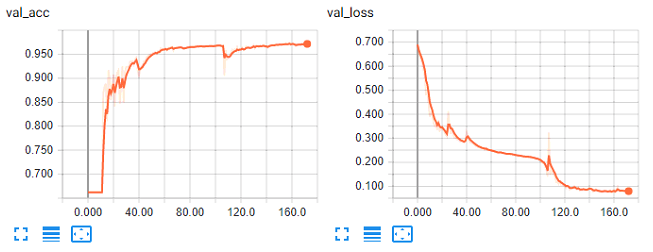
\includegraphics[width=1\textwidth]{bilder/custom_1_training/Custom_1_sequential_val_acc_training_results.png}
\caption{Validation accuracy and loss}
\label{fig:custom_1_sequential_val_acc_result}
\end{subfigure}
\caption{The training and validation set results from the sequential network, trained on the \textit{Custom 1} dataset}
\label{fig:custom_1_sequential_result}
\end{figure}

The training results in \cref{fig:custom_1_sequential_result} are not as smooth as in \cref{fig:custom_1_residual_result}. The curves are a little bit spikier in general in this particular training. Despite the tendency to spiky graphs, no major overfitting is observed during this training of the sequential network.

\begin{figure}[ht]
\centering
\begin{subfigure}[b]{\textwidth}
\centering
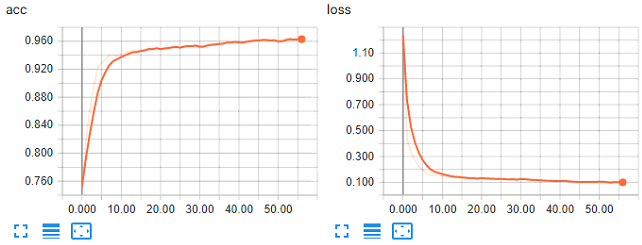
\includegraphics[width=1\textwidth]{bilder/custom_2_training/Custom_2_residual_training_acc_results.png}
\caption{Training accuracy and loss}
\label{fig:custom_2_residual_acc_result}
\end{subfigure}
\hfill
\begin{subfigure}[b]{\textwidth}
\centering
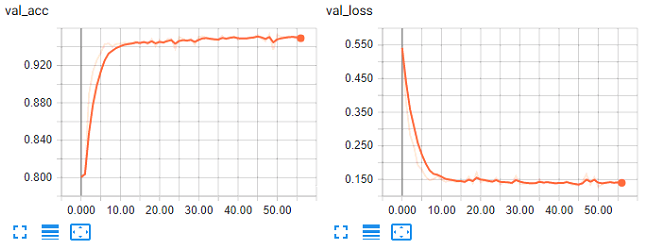
\includegraphics[width=1\textwidth]{bilder/custom_2_training/Custom_2_residual_training_val_acc_results.png}
\caption{Validation accuracy and loss}
\label{fig:custom_2_residual_val_acc_result}
\end{subfigure}
\caption{The training and validation set results from the residual network, trained on the \textit{Custom 2} dataset}
\label{fig:custom_2_residual_result}
\end{figure}

The residual network training with the \textit{Custom 2} dataset is also considered successful. The graphs in \cref{fig:custom_2_residual_acc_result} and \cref{fig:custom_2_residual_val_acc_result} illustrates a high accuracy in both training and validation images. The loss converges at around ten percent in the training images, and approximately 15 \% in the validation pictures and no overfitting is observed. This training result is slightly worse than in the residual network training with the \textit{Custom 1} dataset, but the \textit{Custom 2} dataset consists of more images in both the training and the validation set.

\begin{figure}[ht]
\centering
\begin{subfigure}[b]{\textwidth}
\centering
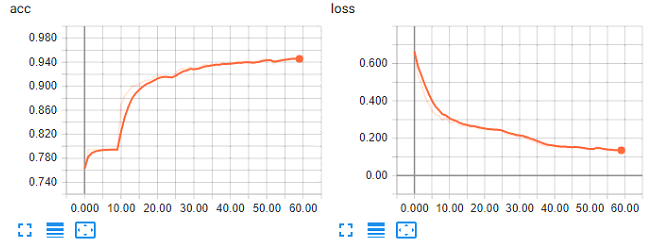
\includegraphics[width=1\textwidth]{bilder/custom_2_training/Custom_2_sequential_training_acc_results.png}
\caption{Training accuracy and loss}
\label{fig:custom_2_sequential_acc_result}
\end{subfigure}
\hfill
\begin{subfigure}[b]{\textwidth}
\centering
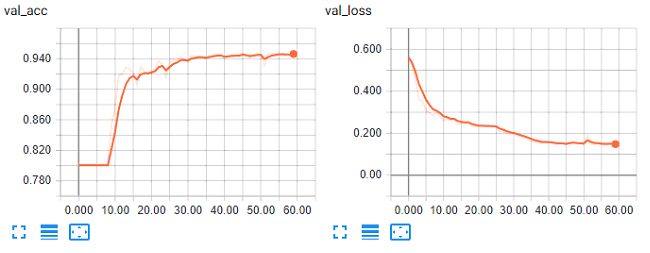
\includegraphics[width=1\textwidth]{bilder/custom_2_training/Custom_2_sequential_training_val_acc_results.png}
\caption{Validation accuracy and loss}
\label{fig:custom_2_sequential_val_acc_result}
\end{subfigure}
\caption{The training and validation set results from the sequential network, trained on the \textit{Custom 2} dataset}
\label{fig:custom_2_sequential_result}
\end{figure}

The last training is the sequential network with the \textit{Custom 2} dataset, illustrated in \cref{fig:custom_2_sequential_result}. This training is quite similar to the previous one except the accuracy is slightly lower, and the loss is barely higher.

\section{Quantitative results}\label{quantitative_results}
This section will provide quantitative results from the three datasets. The result from the \textit{Freiburg Forest} dataset provides the quantitative result from all of the test images in the dataset. As earlier described, a test image is an image the networks have never seen before. The results from the \textit{Custom 1} and the \textit{Custom 2} datasets will only be an indication of the quantitative results. The reason for this is the lack of ground truth in the 2270 test images in total, coming from the two datasets. To be able to make an indication, five uncorrelated images from \textit{Custom 1} dataset, and ten uncorrelated images from \textit{Custom 2} dataset are manually annotated. Then the accuracy, the \ac{iou} for both classes and the \ac{miou} are calculated for each test set. The results are presented in \cref{table:freiburg}, \cref{table:custom_1}, \cref{table:custom_2} and \cref{table:custom_2_2}. The accuracy is described mathematically in \cref{eq:accuracy}.

\begin{equation}\label{eq:accuracy}
\begin{aligned}
Accuracy = \frac{TP + TN}{TP + TN + FP + FN}
\end{aligned}
\end{equation}
Here $TP$, $TN$, $FP$ and $FN$ are true positive, true negative, false positive and false negative respectively. This quantity has a potential weakness in some segmentation problems. If for example one of the classes in a two-class problem, is much larger than the other class, the accuracy might turn out to be higher than it should be. The reason is that both classes are in the equation, and if the much larger class does a useful classification while the other class does not, the accuracy will still be high. To prevent this potential problem, the \ac{iou} metric is included in the tables. The metric is given by \cref{eq:iou}:

\begin{equation}\label{eq:iou}
\begin{aligned}
IoU = \frac{TP}{TP + FP + FN}
\end{aligned}
\end{equation}
Opposite to the accuracy metric, the \ac{iou} only includes one of the two true classifications in a two-class problem. Having only true positives (TP) in the numerator means as briefly described above that this metric might describe each class with a more accurate accuracy in segmentation problems. This is especially applicable when one of the classes is much larger than the other. Imagine the two-class problem in the thesis, where the classes predicted is road and background. If the background is 90 \% of the image and receives a good classification while the road classification receives a bad classification, the accuracy might end up incorrectly too high.

\begin{figure}[ht]
    \centering
    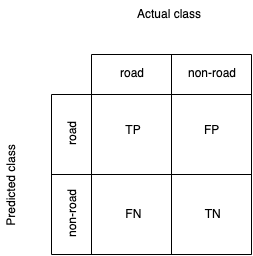
\includegraphics[width=0.35\textwidth]{bilder/confusion_matrix.png}
    \caption{This thesis confusion matrix}
    \label{fig:confusion_matrix}
\end{figure}


\begin{equation}\label{eq:confusion_matrix}
\begin{aligned}
Confusion\:matrix =
\begin{bmatrix} 
   c_{11} & c_{12} \\
   c_{21} & c_{22} \\
\end{bmatrix} 
\end{aligned}
\end{equation}

For a broader understanding on the \cref{eq:iou}, this thesis confusion matrix is introduced in \cref{fig:confusion_matrix} and \cref{eq:confusion_matrix}. In this notation the \textit{non-road} represents the background, and the \textit{actual class} is the ground truth. In \cref{eq:confusion_matrix} the contents of the matrix are substituted. Where $c_{11}$ denote the true positive, $c_{12}$ the false positive, $c_{21}$ is false negative and $c_{22}$ the true negative. In this thesis, the true positive of the confusion matrix is when both the prediction and the ground truth agrees that the pixel is the road. The true negative is when both the prediction and the ground truth agrees that the pixel is the background. The correct classifications from the road and the background will be shown in the diagonal of the matrix respectively ($c_{11}$ and $c_{22}$).

\begin{equation}\label{eq:iou_1}
\begin{aligned}
IoU_{road} = \frac{c_{11}}{c_{11} + c_{12} + c_{21}}
\end{aligned}
\end{equation}

\begin{equation}\label{eq:iou_2}
\begin{aligned}
IoU_{background} = \frac{c_{22}}{c_{22} + c_{21} + c_{12}}
\end{aligned}
\end{equation}

\Cref{eq:iou_1} and \cref{eq:iou_2} describes the \ac{iou} for each of the two classes explicitly. These two equations are the ones that present the \ac{iou} in the following tables. The equations consist of the notation substituted from the confusion matrix. 

\begin{equation}\label{eq:miou}
\begin{aligned}
mIoU = \frac{IoU_{road} + IoU_{background}}{2}
\end{aligned}
\end{equation}

The last metric used for presenting the quantitative results is the \ac{miou}. As described in \cref{eq:miou} it takes the mean of both the \ac{iou} classes. 

\begin{table}[ht]
\centering
\begin{tabular}{lllll}
\hline
 & Accuracy & $IoU_{road}$ & $IoU_{background}$ & mIoU  \\ \hline
Residual network & \quad 98.2\% & \quad 75.9 \% & \quad 98 \%  & 86.9 \%  \\
Sequential network & \quad 89.4 \% & \quad 47\% & \quad 89\% & 67.9\%  \\ \hline
\end{tabular}
\caption{The test set result from the \textit{Freiburg Forest} dataset}
\label{table:freiburg}
\end{table}

The first quantitative results presented in this thesis provide the results from what the two networks managed to predict from the test images with the \textit{Freiburg Forest} dataset. The results is presented in \cref{table:freiburg}. As this is the only quantitative results presented in this thesis which is not just an indication, these results should be considered most accurate in showing the complete accuracy of the dataset. As earlier mentioned \textit{Freiburg Forest} dataset is the only one that contains ground truth for the whole test set. As seen in \cref{table:freiburg}, the residual network does an all over better performance compared to the sequential network. 
\begin{table}[ht]
\centering
\begin{tabular}{lllll}
\hline
 & Accuracy & $IoU_{road}$ & $IoU_{background}$ & mIoU \\ \hline
Residual network & \quad 97.7\% & \quad 92.5\% & \quad  96.6\%  &  94.5\% \\
Sequential network & \quad 98\% & \quad 93.6\% & \quad 97.1\% & 95.3\%  \\ \hline
\end{tabular}
\caption{The test set result from the \textit{Custom 1} dataset}
\label{table:custom_1}
\end{table}

The next quantitative results presented are from the predictions on the \textit{Custom 1} dataset. Since these measurements only come from five uncorrelated images in the test set, the results can only be interpreted as an indication of what the actual quantitative result would be. In this indication, the sequential network performs slightly better than the residual network. Both networks have an overall high accuracy with its predictions on the \textit{Custom 1} dataset. Why the sequential network had a slightly better performance metrics than the residual network will be further discussed in \cref{discussion}.   

\begin{table}[ht]
\centering
\begin{tabular}{lllll}
\hline
 & Accuracy & $IoU_{road}$ & $IoU_{background}$ & mIoU \\ \hline
Residual network & \quad 94.1\% & \quad  77.7\% & \quad 92.7\%  &  85.3\% \\
Sequential network & \quad 94\% & \quad 77.4\% & \quad 92.6\% & 85\% \\ \hline
\end{tabular}
\caption{The test set result from the \textit{Custom 2} dataset}
\label{table:custom_2}
\end{table}

\begin{table}[ht]
\centering
\begin{tabular}{lllll}
\hline
 & Accuracy & $IoU_{road}$ & $IoU_{background}$ & mIoU \\ \hline
Residual network & \quad 90.5\% & \quad  65.2\% & \quad 88.6\%  &  76.9\%  \\
Sequential network & \quad 91\% & \quad 66.3\% & \quad 89.3\% & 77.7\% \\ \hline
\end{tabular}
\caption{The second test set result from the \textit{Custom 2} dataset}
\label{table:custom_2_2}
\end{table}

The last indication of the quantitative results is presented in \cref{table:custom_2} and \cref{table:custom_2_2}, and consists of predictions from the \textit{Custom 2} dataset. The overall results from these two tables are also considered a good result. This dataset has combined 1876 test images, while the amount of training and validation images is 164. The first table shows slightly better results overall, but this is as expected due to the last test set (404 images) being completely independent from the training and validation images.

\section{Qualitative results}
This part will consist of a few qualitative results from both network predictions on all datasets. The results presented in this section consist of good and poor predictions, and predictions from challenging areas due to for example objects in the scene, shadows et cetera. A more extended image sequence from each dataset which can be used to observe the results from the predictions can be found in the appendix.

\begin{figure}[ht]
\centering
\begin{subfigure}[b]{\textwidth}
\centering
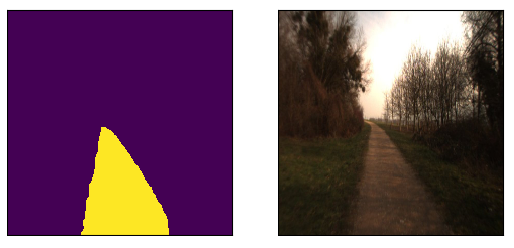
\includegraphics[width=0.8\textwidth]{bilder/freiburg/b57-8406_Clipped_res.png}
\caption{Residual network}
\label{fig:ff_res}
\end{subfigure}
\hfill
\begin{subfigure}[b]{\textwidth}
\centering
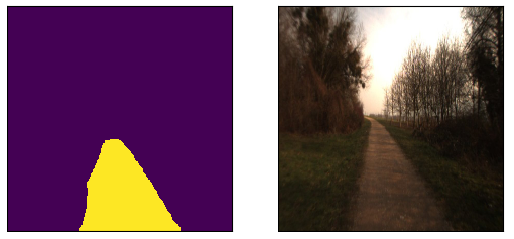
\includegraphics[width=0.8\textwidth]{bilder/freiburg/b57-8406_Clipped_seq.png}
\caption{Sequential network}
\label{fig:ff_seq}
\end{subfigure}
\caption{Two samples from the test set predictions on the
\textit{Freiburg Forest} dataset}
\label{fig:ff_result}
\end{figure}
The first qualitative result comes from the \textit{Freiburg Forest} dataset, and is illustrated in \cref{fig:ff_result}. Comparing the two networks from \cref{fig:ff_res} and \cref{fig:ff_seq}, the residual network gives a more precise prediction of the road than the sequential network. This single result corresponds to the metrics in \cref{table:freiburg}, where the residual network did get better results overall as well. 

\begin{figure}[ht]
\centering
\begin{subfigure}[b]{\textwidth}
\centering
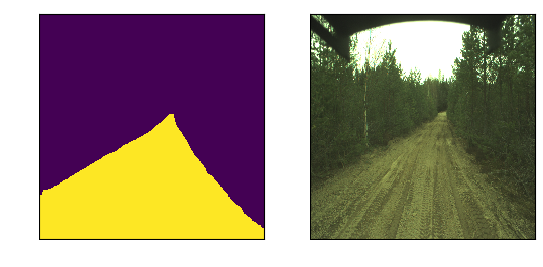
\includegraphics[width=0.8\textwidth]{bilder/custom_1/185_residual.png}
\caption{Residual network}
\label{fig:custom_1_res}
\end{subfigure}
\hfill
\begin{subfigure}[b]{\textwidth}
\centering
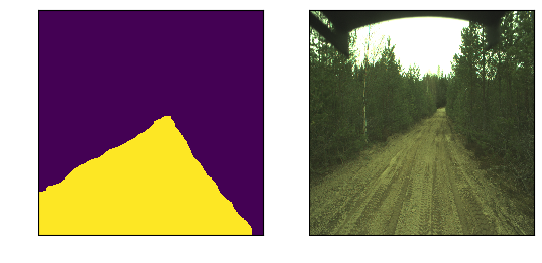
\includegraphics[width=0.8\textwidth]{bilder/custom_1/185_sequential.png}
\caption{Sequential network}
\label{fig:custom_1_seq}
\end{subfigure}
\caption{Two samples from the test set predictions on the
\textit{Custom 1} dataset}
\label{fig:custom_1_result}
\end{figure}

The next two predictions come from the \textit{Custom 1} dataset. Also here, the residual network provide a better prediction on the test set sample than the sequential network. The sequential network stops at predicting the road before the residual network does, in the tip of the road. A slight color change can be seen in that small area, which might explain why. In the indication of the quantitative results shown in \cref{table:custom_1}, the sequential network gave a slightly more accurate result than the residual network, and as seen in \cref{fig:custom_1_result} this does not correspond to the qualitative result were the residual prediction was better. Some theories about this will be discussed in \cref{discussion}. 
%A theory may be that the number of true positives (actual road predicted as the road) in the \ac{iou} metric is much higher than the false negatives (actual road predicted as background). A vast difference between true positives and false negatives can potentially make the metrics provide a good result for the sequential network, even though it contains slightly more false negatives than the residual network. A potentially much higher number of true positives than false negatives makes the \ac{iou} metric almost to ignore small differences in false negatives between the networks. Another theory can be that the few images picked out for the quantitative results indication contained better predictions from the sequential network.

\begin{figure}[ht]
\centering
\begin{subfigure}[b]{\textwidth}
\centering
\includegraphics[width=0.8\textwidth]{bilder/custom_1/361_residual.png}
\caption{Residual network}
\label{fig:custom_1_res_poor}
\end{subfigure}
\hfill
\begin{subfigure}[b]{\textwidth}
\centering
\includegraphics[width=0.8\textwidth]{bilder/custom_1/361_sequential.png}
\caption{Sequential network}
\label{fig:custom_1_seq_poor}
\end{subfigure}
\caption{Two samples from the test set predictions on the
\textit{Custom 1} dataset. Containing a car in the image }
\label{fig:custom_1_result_car}
\end{figure}

\Cref{fig:custom_1_result_car} illustrates two predictions with an object (car) placed in the road. Both networks perform less than normal every time unknown objects arrive in the scene, but the residual network makes a surprisingly good prediction in \cref{fig:custom_1_res_poor} compared to the sequential network. From other examples, it seems like both networks finds it challenging at first when new objects arrive at the scene before they quickly get back to good predictions. The residual network is slightly faster and more robust than the sequential network when it comes to resume good predictions after challenging scenes.
\begin{figure}[ht]
\centering
\begin{subfigure}[b]{\textwidth}
\centering
\includegraphics[width=0.8\textwidth]{bilder/custom_2/474_res.png}
\caption{Residual network}
\label{fig:custom_2_res}
\end{subfigure}
\hfill
\begin{subfigure}[b]{\textwidth}
\centering
\includegraphics[width=0.8\textwidth]{bilder/custom_2/474_seq.png}
\caption{Sequential network}
\label{fig:custom_2_seq}
\end{subfigure}
\caption{Two samples from the test set predictions on the \textit{Custom 2} dataset (The first test set with 1472 images)}
\label{fig:custom_2_result}
\end{figure}

\Cref{fig:custom_2_result} shows two examples of a challenging scene containing shadows, where the networks predict rather well. The large shadow part in the bottom of the images does not seem to concern any of the networks. The overall best prediction in this example comes from the residual network. 

\begin{figure}[ht]
\centering
\begin{subfigure}[b]{\textwidth}
\centering
\includegraphics[width=0.8\textwidth]{bilder/custom_2_exclusive/1938_res.png}
\caption{Residual network}
\label{fig:custom_2_2_res}
\end{subfigure}
\hfill
\begin{subfigure}[b]{\textwidth}
\centering
\includegraphics[width=0.8\textwidth]{bilder/custom_2_exclusive/1938_seq.png}
\caption{Sequential network}
\label{fig:custom_2_2_seq}
\end{subfigure}
\caption{Two samples from the test set predictions on the \textit{Custom 2} dataset (The second test set with 404 images)}
\label{fig:custom_2_result_404}
\end{figure}

\Cref{fig:custom_2_result_404} illustrates a similar challenging scene as the example above in \cref{fig:custom_2_result}. The main difference between the two results is which test set they come from. These samples are taken from the test set which only consists of 404 images, and does not have any correlation to the training and validation images at all. As earlier described, the training and validation images are chosen iteratively from the start to the end of the dataset, meaning, for example, every 100'th in the dataset is chosen for training and validation. This method is chosen due to the desire for automatically predicting the rest of the dataset as annotation for the test images. Unlike the other two test sets, this test set has been left alone and consists of an untouched sequence. Being able to predict a good prediction on such an untouched scene as illustrated in these two images, means the network is somewhat generalized and has the opportunity to predict well on more completely unseen and uncorrelated data as well.

\begin{figure}[ht]
\centering
\begin{subfigure}[b]{\textwidth}
\centering
\includegraphics[width=0.8\textwidth]{bilder/custom_2/154_res_poor.png}
\caption{Residual network}
\label{fig:custom_2_poor_res}
\end{subfigure}
\hfill
\begin{subfigure}[b]{\textwidth}
\centering
\includegraphics[width=0.8\textwidth]{bilder/custom_2/154_seq_poor.png}
\caption{Sequential network}
\label{fig:custom_2_poor_seq}
\end{subfigure}
\caption{Two poor test set prediction from the \textit{Custom 2} dataset (The first test set with 1472 images)}
\label{fig:custom_2_poor}
\end{figure}

These two predictions illustrated in \cref{fig:custom_2_poor} are examples of a challenging scene for the networks. The scene is from a U-turn made by the vehicle, and there is not a structured line in the road as it consists of frequently small areas with grass. The accuracy of the prediction in these particular scenes is, therefore, more reduced than in the rest of the datasets. The difference between the residual and the sequential network is also here noticeable. Once again the residual network shows slightly better results.


\chapter{Discussion and conclusion}\label{discussion}
This chapter will first examine the quantitative and then the qualitative results presented in the thesis. The next section will provide an analyze of the use of transfer learning and discuss challenging scenes from the images. Then the next part will discuss the quality of the manually annotated images and the generating of the training and the validation sets. Lastly, this chapter will conclude the thesis and provide suggestions for further work. 

The chapter will answer the goals which not yet has been answered by \cref{method}. The goals which also are described in the introduction are as follows: 
\begin{itemize}
    \item \textbf{Perform a literature review of existing \acp{cnn} and choose a robust network to implement}
    \item \textbf{Implement a very basic \ac{cnn} in addition, to use as baseline}
    \item \textbf{Investigate if the \acp{cnn} predictions are good enough to be used as ground truth for the images in the datasets}
    \item \textbf{Gain a more generalized network with transfer learning from a similar dataset}
    \item \textbf{Make two different versions of the training set}
    \item \textbf{Test the networks, present the results, and analyze them}
\end{itemize}

\section{Quantitative results}
It is necessary to have ground truth in all of the test images, respectively, to calculate the quantitative results. The only dataset with ground truth for all test images is as earlier described the dataset from the University of Freiburg. Consequently is the \textit{Freiburg Forest} dataset the only one that gets the actual quantitative results from the networks in this task, and therefore, should these quantitative results be emphasized most. The results was presented in \cref{quantitative_results} from \cref{table:freiburg}. As seen in \cref{table:freiburg}, the residual outperforms the sequential network in all metrics, as expected. The scene in the \textit{Freiburg Forest} dataset contains several challenging areas to predict, like for example narrow roads, sunshine, and much grass in the path. These challenging scenes appear more often in the \textit{Freiburg Forest} dataset than in the \textit{Custom 1} and \textit{Custom 2} dataset, and may be one of the reasons for the residual networks greater performance. 

As earlier mentioned, the quantitative results from the \textit{Custom 1} and the \textit{Custom 2} dataset will only be an indication of a quantitative result. The reason for only indicating a quantitative result is due to the time cost of producing manually labeled images, as none are included in the test set. Five uncorrelated images are chosen from the test set to be manually annotated, and the metrics are then calculated in a small script. The results presented in \cref{table:custom_1} describes the two networks quantitative results from the test images in the \textit{Custom 1} dataset. Compared to the \textit{Custom 2} with its 2040 images, the \textit{Custom 1} dataset has only 439 images in total. The quantitative result from \cref{table:custom_1} shows an overall high accuracy from both networks. The high accuracy from both networks is the desired result. As seen in \cref{table:custom_1}, the sequential network has overall slightly higher accuracy than the residual network, and this is not as excepted since the residual network should be the better one. A reason for the slightly better accuracy in the sequential network may be that the images picked out from the test set contained the best predictions from the sequential network, while the best from the residual network was not included. Another theory can be that the $FP$ and the $FN$ values vary between the networks. Low $FP$ and high $FN$ values from the first network, and opposite values in the form of respectively correlated high $FP$ and low $FN$ values in the second network might provide similar \ac{iou} accuracy. $FP$ is the predictions where the network falsely think it is road, and $FN$ is the predictions where the network falsely think it is the background. The most unwanted scenario is where the $FP$ values are too high because it is not desired to have a falsely predicted road where it is no road. The residual network had $FP=156\ pixels$ and $FN=994\ pixels$, while the sequential network had $FP=534\ pixels$ and $FN=439\ pixels$ in the \textit{Custom 1} dataset. The mean values from the actual road are $TP=14828\ pixels$, while the mean actual background values are $TN=34215\ pixels$. Put in context, the values from $FP$ are low compared to $TP$, which means there is only a tiny fraction of the image, which is falsely predicted as the road. Since the $FP$ values from the residual network are lower than from the sequential network, it may indicate that the results from the residual network are better, despite the slightly higher accuracy in \cref{table:custom_1} from the sequential network. 

The two last indications of quantitative results is presented in \cref{table:custom_2} and \cref{table:custom_2_2}, and comes from two different test set in the \textit{Custom 2} dataset. The metrics are calculated from ten manually annotated images in the first test set, and five manually labeled images from the second test set, all images without correlation to each other. The results in \cref{table:custom_2} and \cref{table:custom_2} are slightly lower than in \cref{table:custom_1}, but this is as expected since the \textit{Custom 2} dataset consists of totally 2040 images with occasionally a more challenging scene. 

As seen in the quantitative results from \cref{table:freiburg}, the residual network was better than the sequential network. If it had been ground truth for all test images in the \textit{Custom 1} and the \textit{Custom 1} dataset, may the likelihood exist for seeing the same pattern in the networks quantitative results from these datasets as well. The reason to anticipate this outcome is supported further in the qualitative results presented, where it is illustrated that the predictions from the sequential network are poorer than the residual network's predictions in more challenging scenes. 

\section{Qualitative results}
The most expedient results to interpret in this thesis are the qualitative results since they provide a clear, explicit illustration of the quality of the predictions from the networks. As there may be several reasons for the quantitative results to provide falsely high accuracy in some occasions, the qualitative results presented as images with predicted ground truth gives a better understanding if the prediction fulfills the users' requirements. As illustrated in \cref{fig:custom_1_result}, the residual network makes overall better predictions than the sequential network, and similar examples of the same outcome will be illustrated in the appendix under \cref{appendix_1}. Providing overall better predictions than the sequential network, the residual network is the most robust network in this thesis. Its predictions have high accuracy in the most scenes in the \textit{Custom 1} and \textit{Custom 2} datasets testing images.        

\section{Transfer learning}
Before implementing the transfer learning from the networks training on the \textit{Freiburg Forest} dataset, the predictions from both networks were a little inadequate on the two custom datasets. These predictions missed a little bit more of the road areas close to the trenches. The features the two networks learned from the \textit{Freiburg Forest} datasets 207 training images from a similar environment as in the \textit{Custom 1} and \textit{Custom 2} dataset, helped improved the overall accuracy in the predictions. For that reason, transfer learning from a similar dataset may be considered a good idea, and it proved to give slightly more generalized networks in this thesis.  

\section{Challenging scenes}
The \textit{Custom 1} and \textit{Custom 2} dataset contains several images with a challenging scene for the semantic segmentation problem in this thesis. The first one is presented in \cref{fig:custom_1_result_car}, where a car arrives at the top left position in the image. Since this thesis only handles a two-class problem, it was uncertain how the networks would react to a car in the scene. \Cref{fig:custom_1_result_car} shows that the residual network managed to get a good prediction, while the sequential network predicted the image with slightly lower accuracy.

Another demanding scene is presented in \cref{fig:custom_2_result}, where the road consists of shadows. In traditional \ac{ml} problems, a scene like this may cause a poorer prediction due to the color change from the shadows, but both the residual and the sequential network managed to predict a reasonably good ground truth for the image. The residual network also has here a slightly more accurate prediction.

The last type of challenging scene which was presented in the result chapter was \cref{fig:custom_2_poor}. The image illustrates a U-turn made by the vehicle were the road is partly filled with grass. This type of environment proved to be the most demanding for both networks. Even though the residual network had the best prediction of the two networks, it was not a particularly accurate road prediction. Some of the reasons for this poor prediction may be the lack of either a similar image, including ground truth in the training set or the weak lines in the road due to the grass in the scene. 

Even though the result chapter illustrates some images from challenging scenes with variable accuracy on the predictions, did the two networks provide overall good results in the most predictions as will be illustrated in \cref{appendix}. These examples show that the residual network is slightly more robust than the sequential network in both the more challenging scenes and the ordinary scenes. A method which may increase the robustness and accuracy in all scenes, even more, is implementing several classes. If there would be classes for the most common objects which arrive in the datasets scene, this could help the networks considerably to predict more accurate when these objects arrive. It will require more work on the manual annotation part in the images from the training and validation set, but it is likely to result in better predictions in scenes with these objects. 

\section{The few manually annotated images from the \textit{Custom 1} and \textit{Custom 2} datasets}
As illustrated in \cref{table:dataset} the \textit{Custom 1} dataset consists of 45 manually annotated images from the training and validation set, while the \textit{Custom 2} dataset consists of 164 images. That makes the total number of manually labeled images used for training and validation, 209 images. These are the images that are used to train the two networks, and further potentially automatically produce ground truth for up to 2270 test images from the two datasets. To have these manually annotated images labeled correctly is therefore essential to have the highest chance of successful predictions. The average time spent on manually label each of these training and validation images is around two minutes, which implies that some of the annotations might have the opportunity for improvement. Since the result from the residual network's predictions has decent accuracy, it suggests that the manually labeled images are to some extent accurate enough.          

\section{Generating the training and validation set}
Since the two custom datasets only contain raw images initially, each dataset needs to be split into a training, a validation and a test set. The dataset structure is briefly described in \cref{datasets}, and the training set is the first one which is generated. Depending on the networks goals, it is several ways to generate the training set. In this thesis, the goal is to make the network predict the ground truth for the test images, therefore it makes sense that the training images are from almost similar scenes as the test set images. This is why every tenth image ranging from the beginning to the end of the dataset (in the \textit{Custom 1} and the \textit{Custom 2} datasets) is chosen as the training set. The remaining images in both datasets are chosen to be in the test set. The validation set is generated by taking ten percent of the images from the training set. Having a training set which is slightly correlated to the test images may increase the chances for better predictions in the two custom datasets. \Cref{fig:custom_1_result}, \cref{fig:custom_1_result_car}, \cref{fig:custom_2_result} and \cref{fig:custom_2_poor} are examples of predictions from test sets which is slightly correlated to the training set. All these result with the exception of the \cref{fig:custom_2_poor} are considered decent predictions from the residual network, and slightly poorer but still okay predictions from the sequential network. These results indicates that generating a training set this way works if the goal is to find the ground truth in a test set with slightly correlated images to the training set. 

There is however generated a second test set in the \textit{Custom 2} dataset consisting of 404 images, which are split from the dataset before the training set was created. Having the second test set split before the training set was generated means it may be completely uncorrelated from the training images. The reason this second test set is created is to check if the networks are generalized and can perform well on completely uncorrelated data. A result from this test set is presented in \cref{fig:custom_2_result_404} and the prediction from the residual network is surprisingly decent, considering that the test set is entirely uncorrelated with the training set.         

\section{Conclusion}
Supervised learning with \acp{cnn} is a powerful tool for gaining desired features from images. To apply supervised learning to, for example, a semantic segmentation problem, the dataset needs ground truth for the images. Providing the dataset with ground truth is a time-consuming task, and many raw datasets do not include any ground truth for the images at all. This thesis has two raw datasets with terrain-images and seeks to partly automate the task of producing the ground truth for almost all of these images. The idea is to manually label just a few of the raw images, and use the networks for producing the remaining labels to the images. The problem formulation in this thesis described in the introduction is, therefore:
\begin{itemize}
\centering
  \item[] \textbf{Will the use of \acp{cnn} provide useful test set predictions in a raw terrain-image dataset, given only a few manually annotated images?} 
\end{itemize}
In this thesis, two networks are implemented which purpose is to make the road and background predictions from the test set as detailed so they can be used as ground truth for these images, with only a few images for the network to train on. If the networks manage to do this, potentially an enormous amount of time can be saved instead of manually annotate all the images in the dataset. 

After testing the two networks, and presenting some of the prediction results in \cref{result} and \cref{appendix}, it can be concluded that most of the residual network's predictions can be used as ground truth for the test images in some extent. This means that predictions from the test images with the exceptions of the most demanding scenes can, to some degree, be used as ground truth. The best predictions would be as good as the manually labeled ones, while the remaining predictions would be close to as good, also here except the predictions from the most demanding scenes. The residual network managed to perform consistently better than the sequential network, which was implemented as a baseline. Even though the sequential network managed to deliver similar or slightly better results in the indication of quantitative results, the qualitative results revealed that the residual network proved to be more accurate and robust. The work in this thesis will hopefully be useful to other projects which wish to automate the task of producing ground truth to the images in their raw dataset.

\subsection{Further work}
The suggestions in this section are ideas that have appeared along the way in the late part of the thesis, which, unfortunately, has not been checked out due to the lack of time. Even though the residual network managed to provide many useful predictions, there is always room for improvement. The first suggestion for improving the predictions and making the networks more robust would be to add more classes in the annotated images. As earlier described, including other classes, which have a high probability for arriving in the scene, can contribute to making the networks more robust in these challenging scenes. It will take a little bit more time to annotate each image used for training manually, but may be worth the extra time. To use slightly more time in general on each manual annotation can also be a good idea, to make sure the ground truth for the training images is 100\% accurate.

Another task would be to perform more tweaking of the hyperparameters such as the number of epochs during training, the momentum, resizing the images, test other optimizers than adam, the learning rate, and the regularization. Testing out different hyperparameters can be a repetitive task, but may provide increasingly better results instantaneously, which is rewarding.   

The last suggestion for further work is to check out if the implementation of an active learning algorithm would be able to improve the results even more. The idea would be to use the stream-based selective sampling method. This method takes each unlabeled image and predicts each one at a time, while the algorithm evaluates the informativeness of each image against their query parameter. Further, the user can decide whether to keep or reject the predictions and rerun the process with the accepted predictions added to the training set.

\begin{appendices}
\chapter{Image sequences from the predictions in each dataset}\label{appendix}
\section{Predictions from the \textit{Freiburg Forest} dataset}\label{appendix_freiburg}
\section{Predictions from the \textit{Custom 1} dataset}\label{appendix_1}
\section{Predictions from the \textit{Custom 2} dataset}\label{appendix_2}
\todo{sett inn bildesekvenser av kvalitative prediksjoner}
\end{appendices}

\backmatter{}
\printbibliography
\end{document}
